%\mbox{}\newpage
\chapter{\hspace{-1mm}\bf 数值实验}
\label{chap6}
\addcontentsline{toe}{chapter}{{{\bf Chapter \currentchapter \ 
Numerical Experiments }}\numberline\,}
\markboth{第 \currentchapter \ 章\ \ 
数值实验}{北京航空航天大学博士后研究工作报告}

%%%%%%%%%%%%%%%%%%%%%%%%%%%%%%%%%%%%%%%%%%%%%%%%%%%%%%%%%%%

本章对本报告前面几个章节介绍的部分联邦学习算法进行数值上的评测。评测主要从算法的整体效果 (在测试集上的准确度、损失,以及收敛速度等);对于子节点参与联邦训练比例的鲁棒性;以及对学习率等超参数的敏感性等几个方面进行。为了排除随机因素的干扰,每一组实验都使用了5个不同的随机数种子 (一般都被设为$0, 1, 2, 3, 4$) 进行重复试验,最后得到结果的形式的是均值曲线$\pm$误差界,误差界在这里选取的是标准差。

由于本报告成文时间的关系,本章的数值试验大部分使用的是上一章\S\ref{sec:chap5-datasets}中介绍的小规模的联邦数据集\texttt{FedProxFEMNIST}。选择这个数据集是基于如下的原因:
\begin{itemize}
    \item \texttt{FedProxFEMNIST}数据集来源自真实数据集EMNIST\cite{cohen2017emnist},后者被广泛采用为测试机器学习模型的基准数据集。
    \item \texttt{FedProxFEMNIST}数据集的数据分割方式使得子节点之间的数据是非独立同分布的,而且天然形成了10个聚落的结构,方便评测聚类联邦学习算法\cite{Ghosh_2022_cfl, Sattler_2021_cfl}在内的多种联邦学习算法的鲁棒性。
    \item \texttt{FedProxFEMNIST}数据集的数据规模较小,非常适合联邦学习算法的快速验证工作。
\end{itemize}

%%%%%%%%%%%%%%%%%%%%%%%%%%%%%%%%%%%%%%%%%%%%%%%%%%%%%%%%%%%

\section{联邦学习算法整体效果的数值评测}
\addcontentsline{toe}{section}{{\currentchapter .1\ \ Numerical Evaluation of the Overall Effectiveness of Federated Learning Algorithms}\numberline\,}
\label{sec:chap6-overall}

% almost finished

本节对几种典型的联邦学习算法进行数值上的评测,包括
\begin{itemize}
    \item \texttt{FedAvg}\cite{mcmahan2017fed_avg} (作为\texttt{FedOpt}\cite{reddi2020fed_opt}的特例),
    \item \texttt{FedAdam}\cite{reddi2020fed_opt, adam} (作为\texttt{FedOpt}\cite{reddi2020fed_opt}的特例),
    \item \texttt{FedAdagrad}\cite{reddi2020fed_opt, adagrad} (作为\texttt{FedOpt}\cite{reddi2020fed_opt}的特例),
    \item \texttt{FedYogi}\cite{reddi2020fed_opt, Zaheer_2018_yogi} (作为\texttt{FedOpt}\cite{reddi2020fed_opt}的特例),
    \item \texttt{FedProx}\cite{sahu2018fedprox},
    \item \texttt{Ditto}\cite{li_2021_ditto},
    \item \texttt{FedSplit}\cite{pathak2020fedsplit},
    \item \texttt{IFCA}\cite{Ghosh_2022_cfl},
    \item \texttt{ProxSkip}\cite{proxskip}.
\end{itemize}
各个算法的超参数的设置基本与本报告\S\ref{sec:chap5-design}中展示的典型的联邦学习仿真系统\texttt{fl-sim}命令行接口配置文件\ref{lst:fl-sim-config}~一致,即整体进行100轮次的迭代循环;在每一轮循环内,子节点以步长0.03执行10步子问题迭代训练,训练数据的批大小 (Batch Size)\index{批大小, Batch Size} 采用数据集\texttt{FedProxFEMNIST}预置的默认批大小,值为20.

图\ref{fig:standard-test-ratio-10-val-acc}~是以上列出的几种联邦学习优化算法在在子节点训练参与率为$10\%$ (或者等价地,子节点掉队 (Straggler) 几率为$90\%$) 的场景下,在数据集\texttt{FedProxFEMNIST}的测试集上的准确率曲线。可以看到\texttt{FedOpt}相关的几种算法:\texttt{FedAdam}, \texttt{FedAdagrad}, \texttt{FedYogi}, 包括\texttt{FedAvg},在这种比较极端的场景下,都有非常不错的鲁棒性。除此之外,\texttt{IFCA}, \texttt{Ditto}等算法在这种场景下的鲁棒性也不错。而联邦临近算法\texttt{FedProx}在这种场景下的模型准确率曲线波动比较剧烈,而且在整体100轮的迭代之后还未收敛。\texttt{ProxSkip}以及\texttt{FedSplit}算法在子节点训练参与率为$10\%$的场景下发散。

\begin{figure}[H]
    \centering
    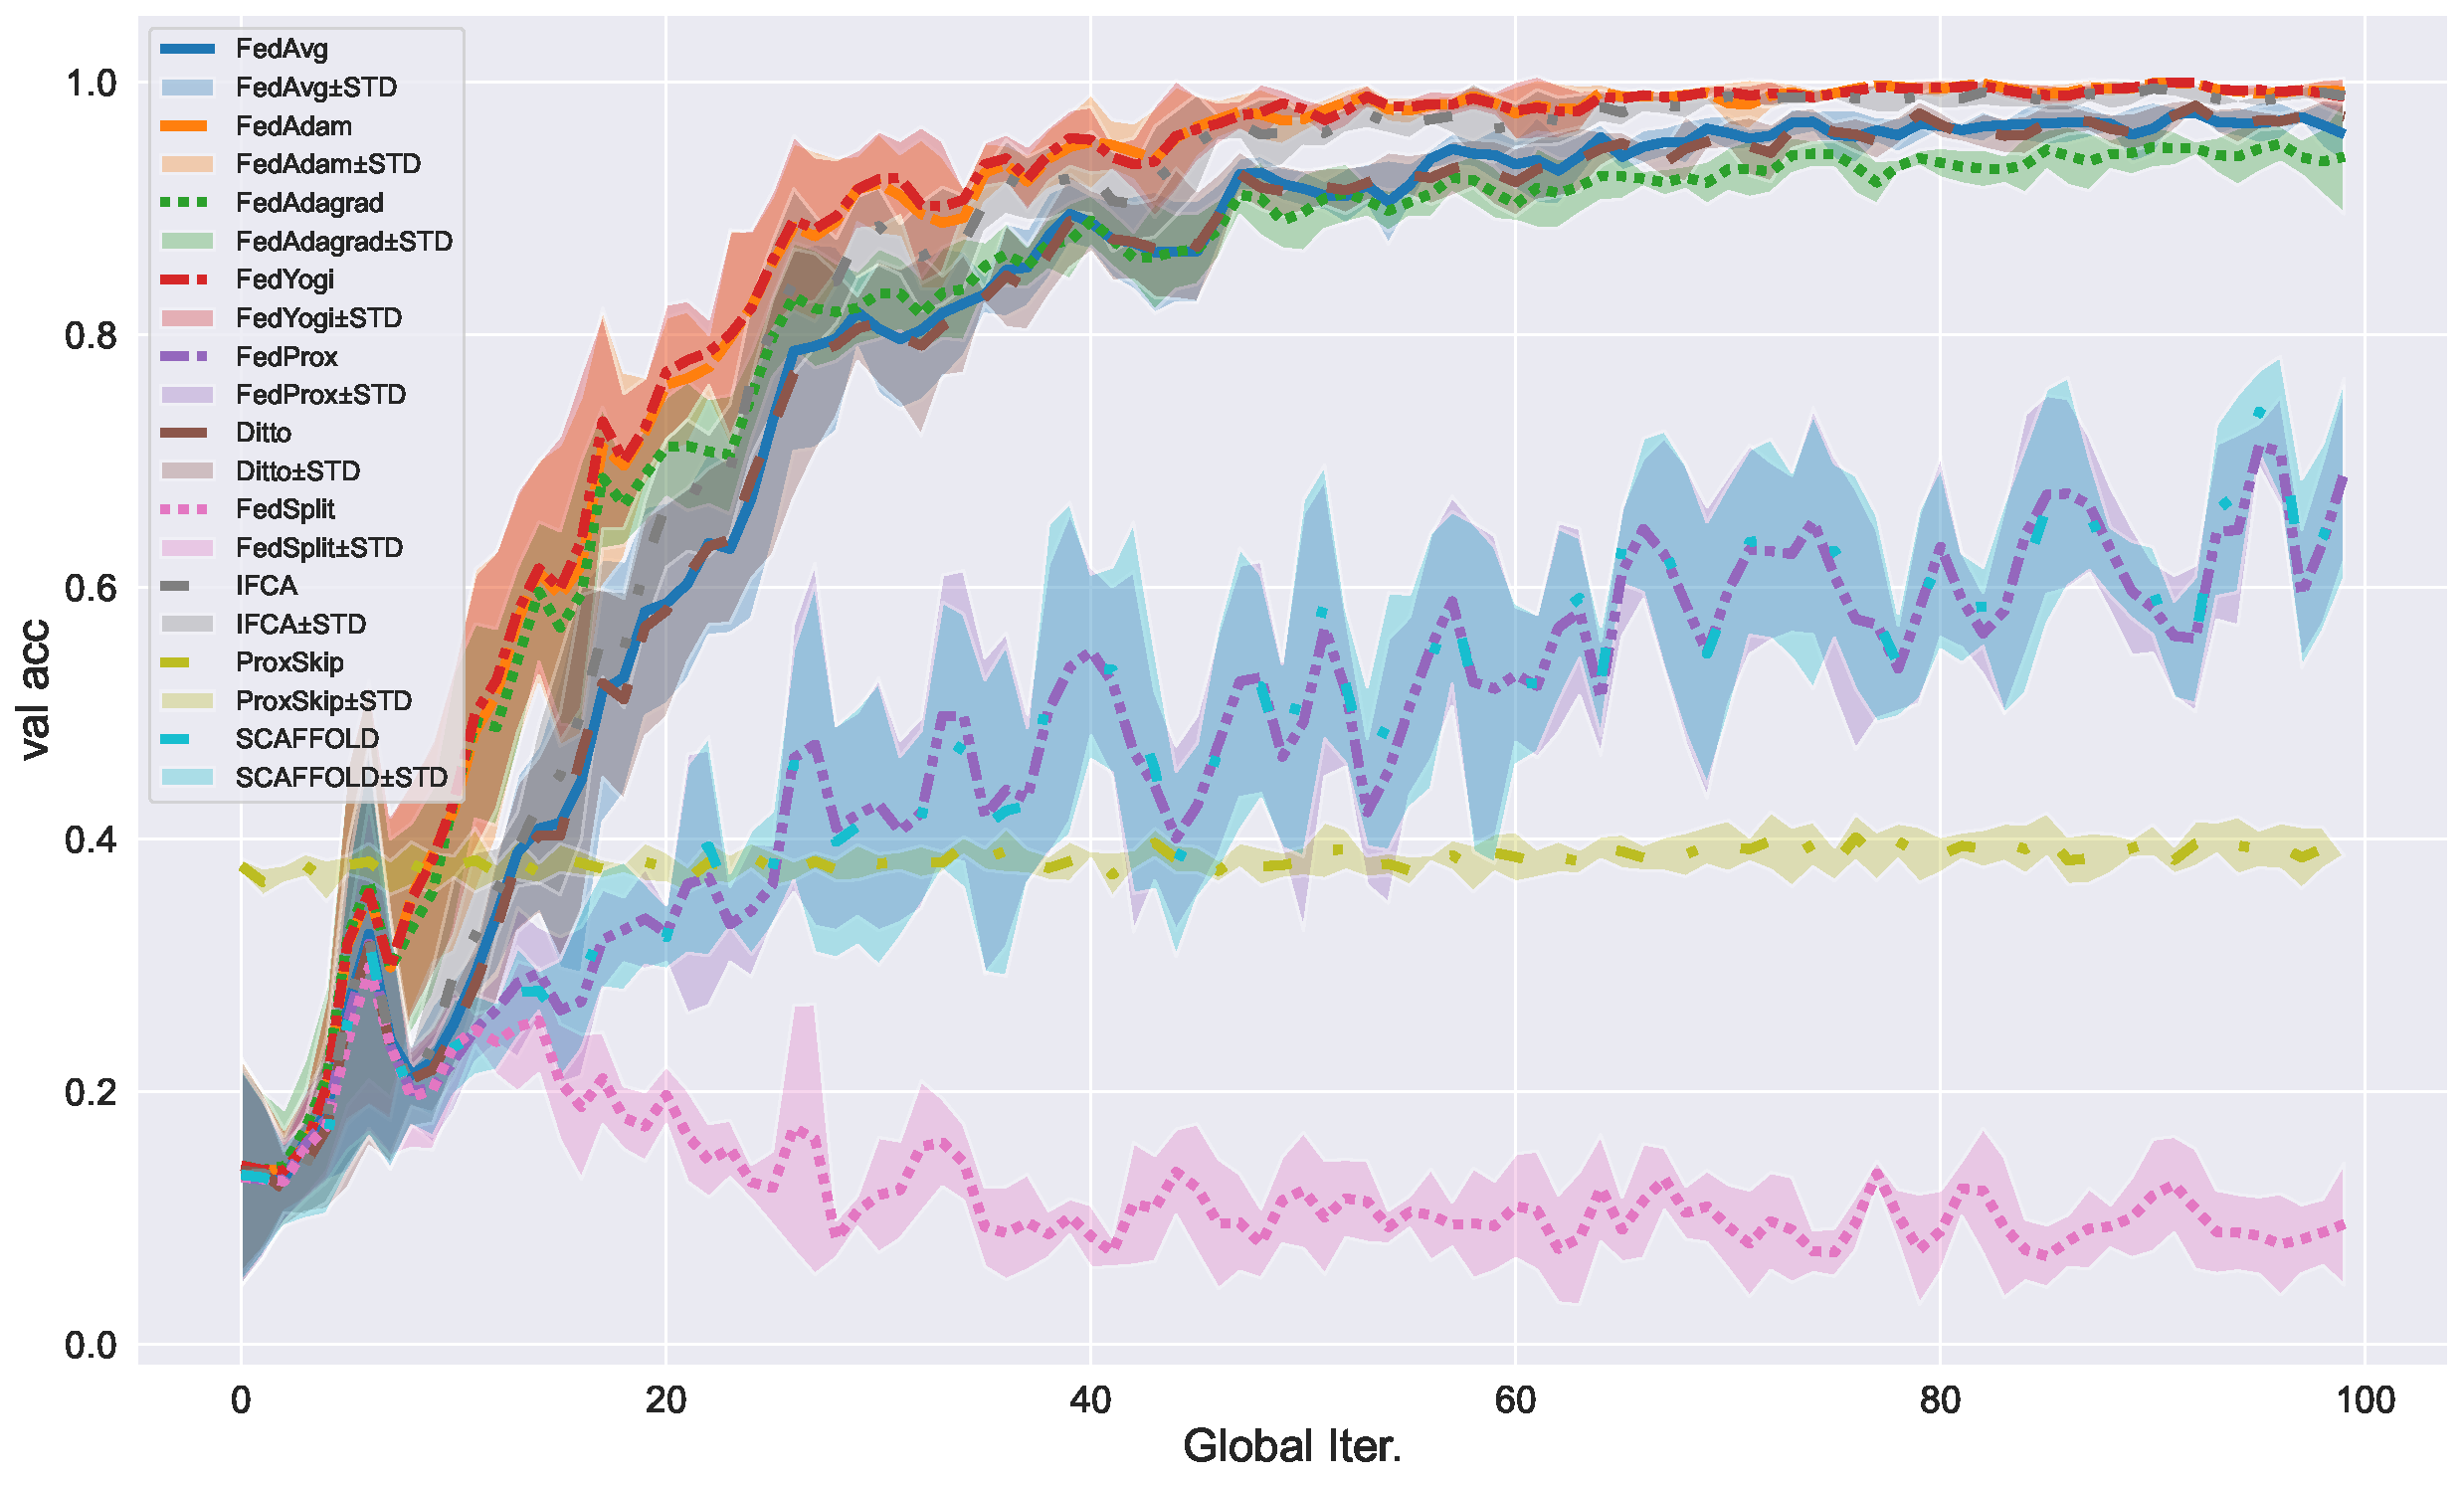
\includegraphics[width=0.9\textwidth]{figures/standard-test-ratio-10-val-acc.pdf}
    \caption{几种典型的联邦学习算法在子节点训练参与率为$10\%$时,在测试集上的准确率曲线}
    \label{fig:standard-test-ratio-10-val-acc}
\end{figure}

图\ref{fig:standard-test-ratio-30-val-acc}, \ref{fig:standard-test-ratio-70-val-acc}, \ref{fig:standard-test-ratio-100-val-acc}~分别是这几种联邦学习优化算法在在子节点训练参与率为$30\%,$ $70\%,$ 以及$100\%$时,在数据集\texttt{FedProxFEMNIST}的测试集上的准确率曲线。可以看到,随着每轮参与训练的子节点比例的提升,或者等价地,每一轮子节点掉队比例的降低,包括\texttt{FedProx}, \texttt{ProxSkip}在内的联邦学习优化算法的稳定性是逐渐提升的,而这其中\texttt{ProxSkip}算法受到的影响是更大的。对于联邦分裂算法\texttt{FedSplit}来说,只有当子节点训练参与率为$100\%$时才不发散,而且在这种情况下,其收敛速度也较慢。

\begin{figure}[H]
    \centering
    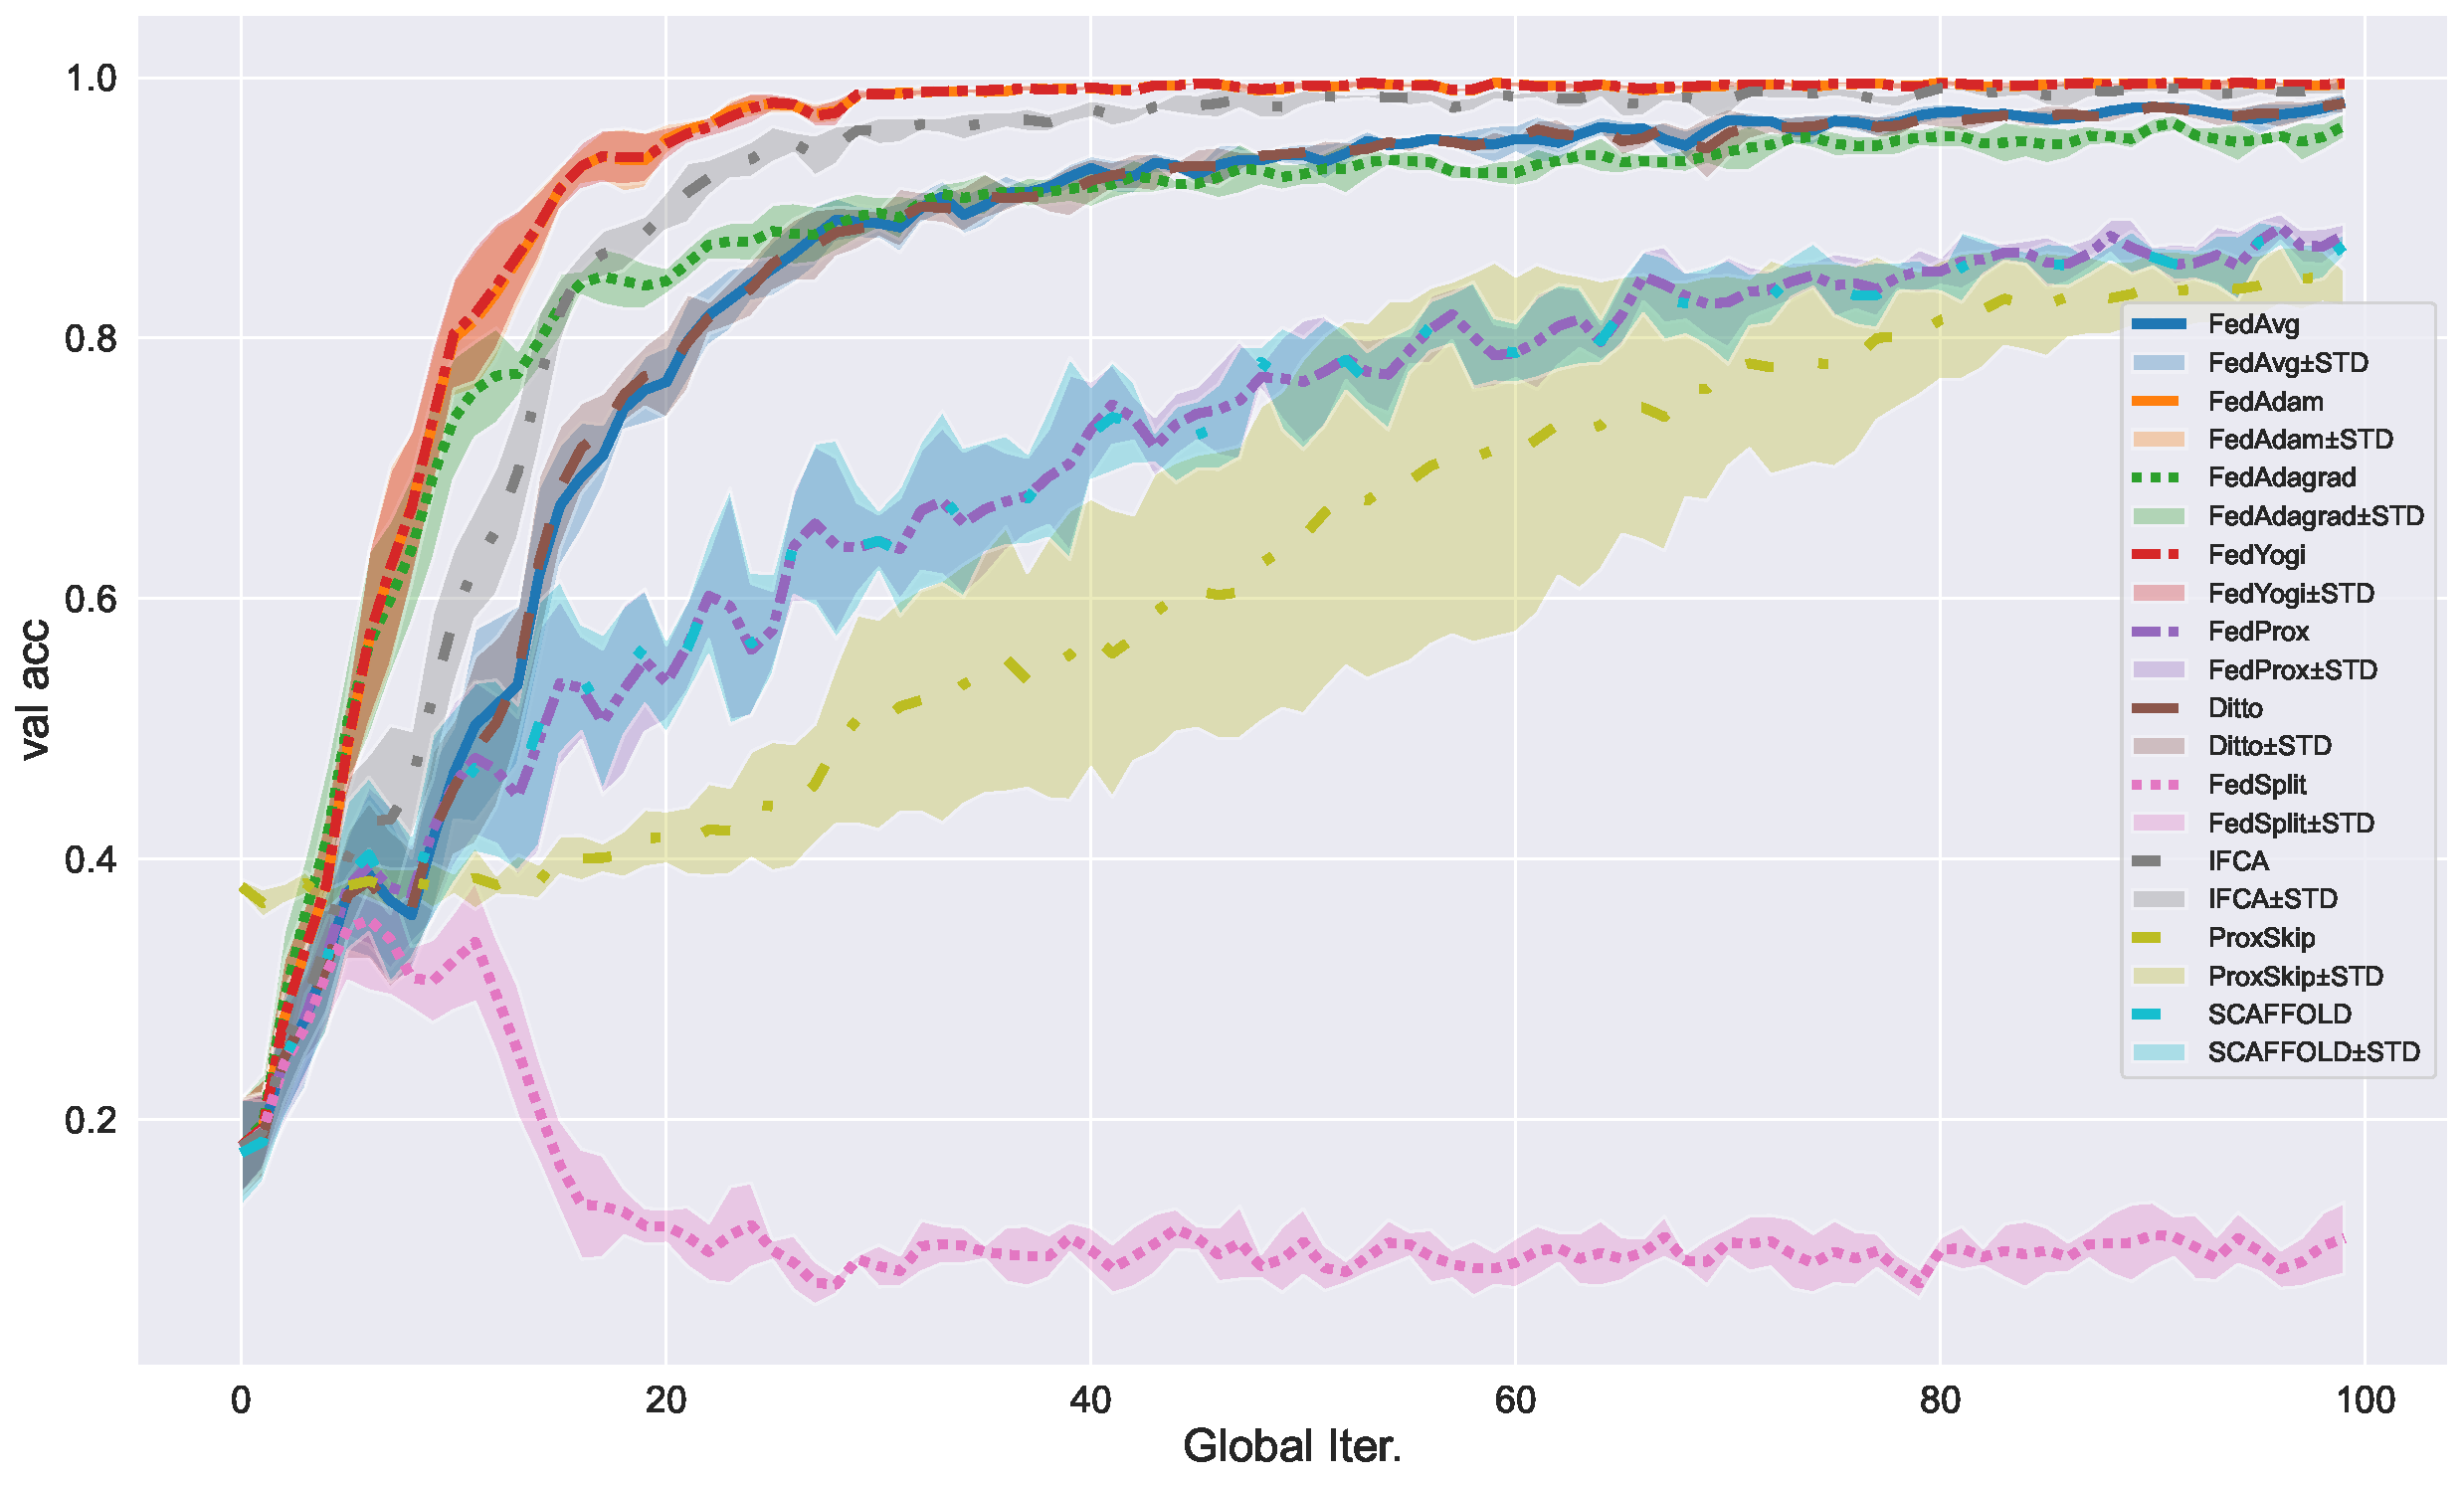
\includegraphics[width=0.9\textwidth]{figures/standard-test-ratio-30-val-acc.pdf}
    \caption{几种典型的联邦学习算法在子节点训练参与率为$30\%$时,在测试集上的准确率曲线}
    \label{fig:standard-test-ratio-30-val-acc}
\end{figure}

\begin{figure}[H]
    \centering
    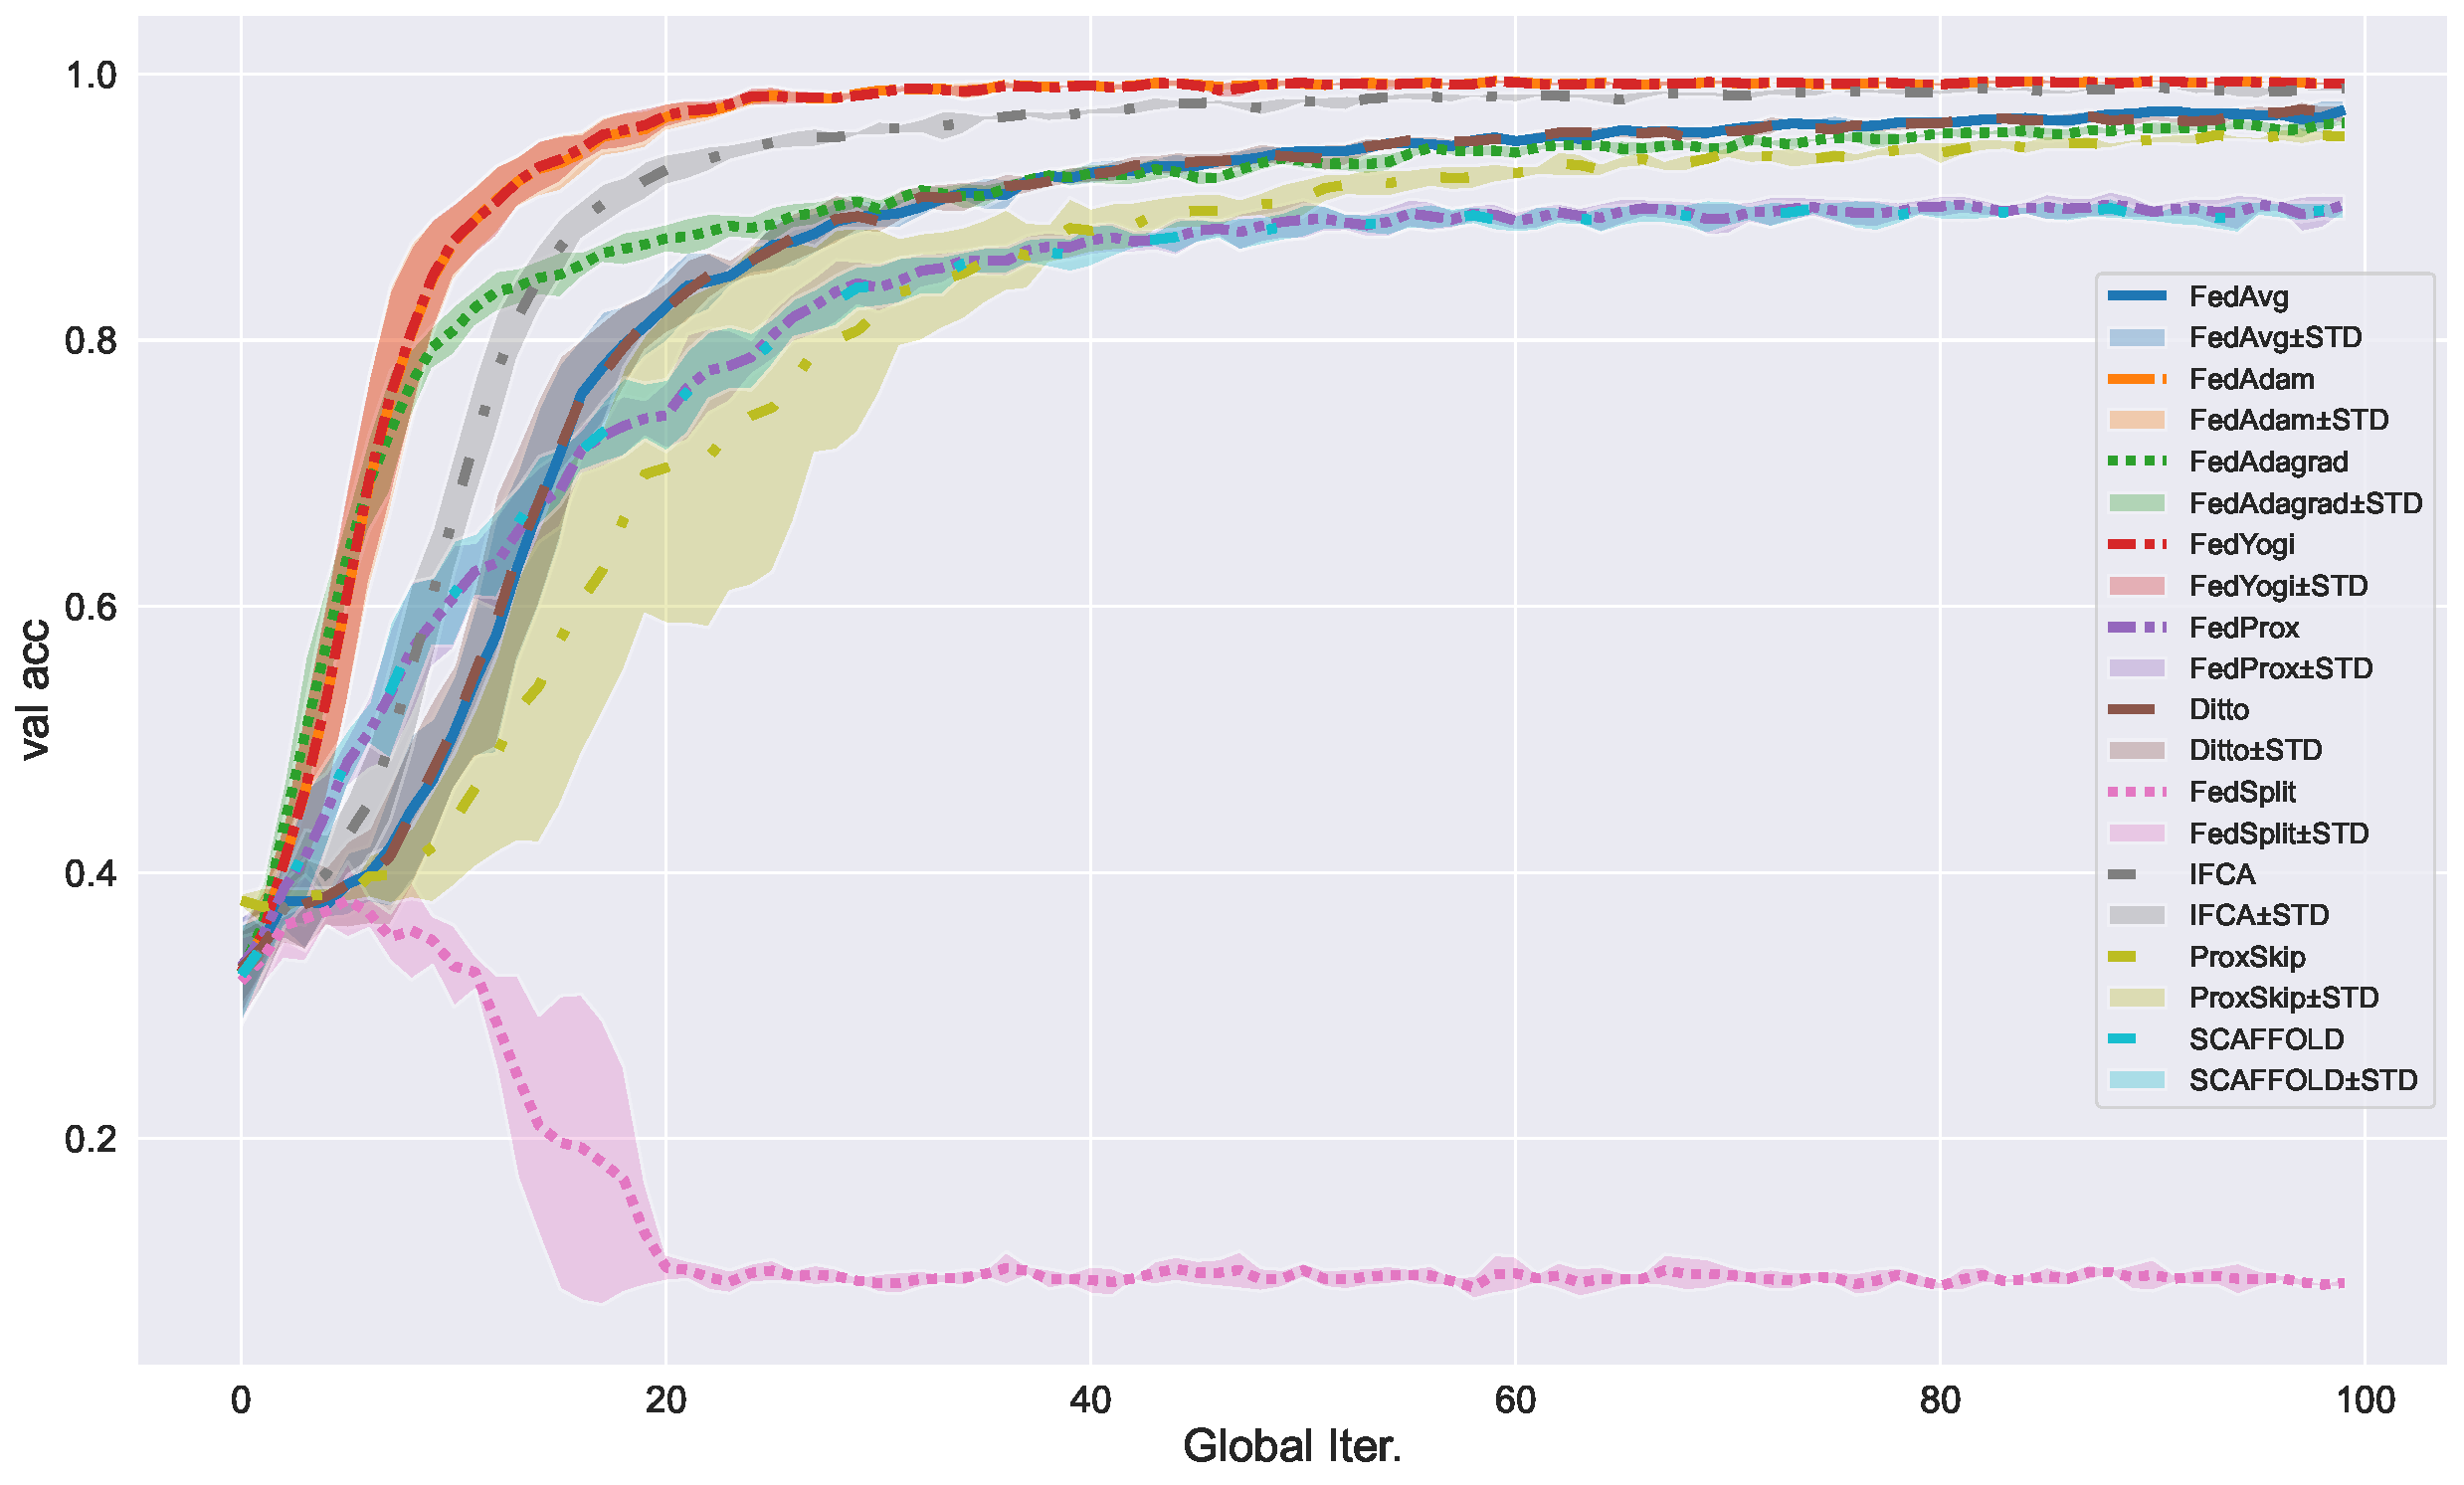
\includegraphics[width=0.9\textwidth]{figures/standard-test-ratio-70-val-acc.pdf}
    \caption{几种典型的联邦学习算法在子节点训练参与率为$70\%$时,在测试集上的准确率曲线}
    \label{fig:standard-test-ratio-70-val-acc}
\end{figure}

\begin{figure}[ht]
    \centering
    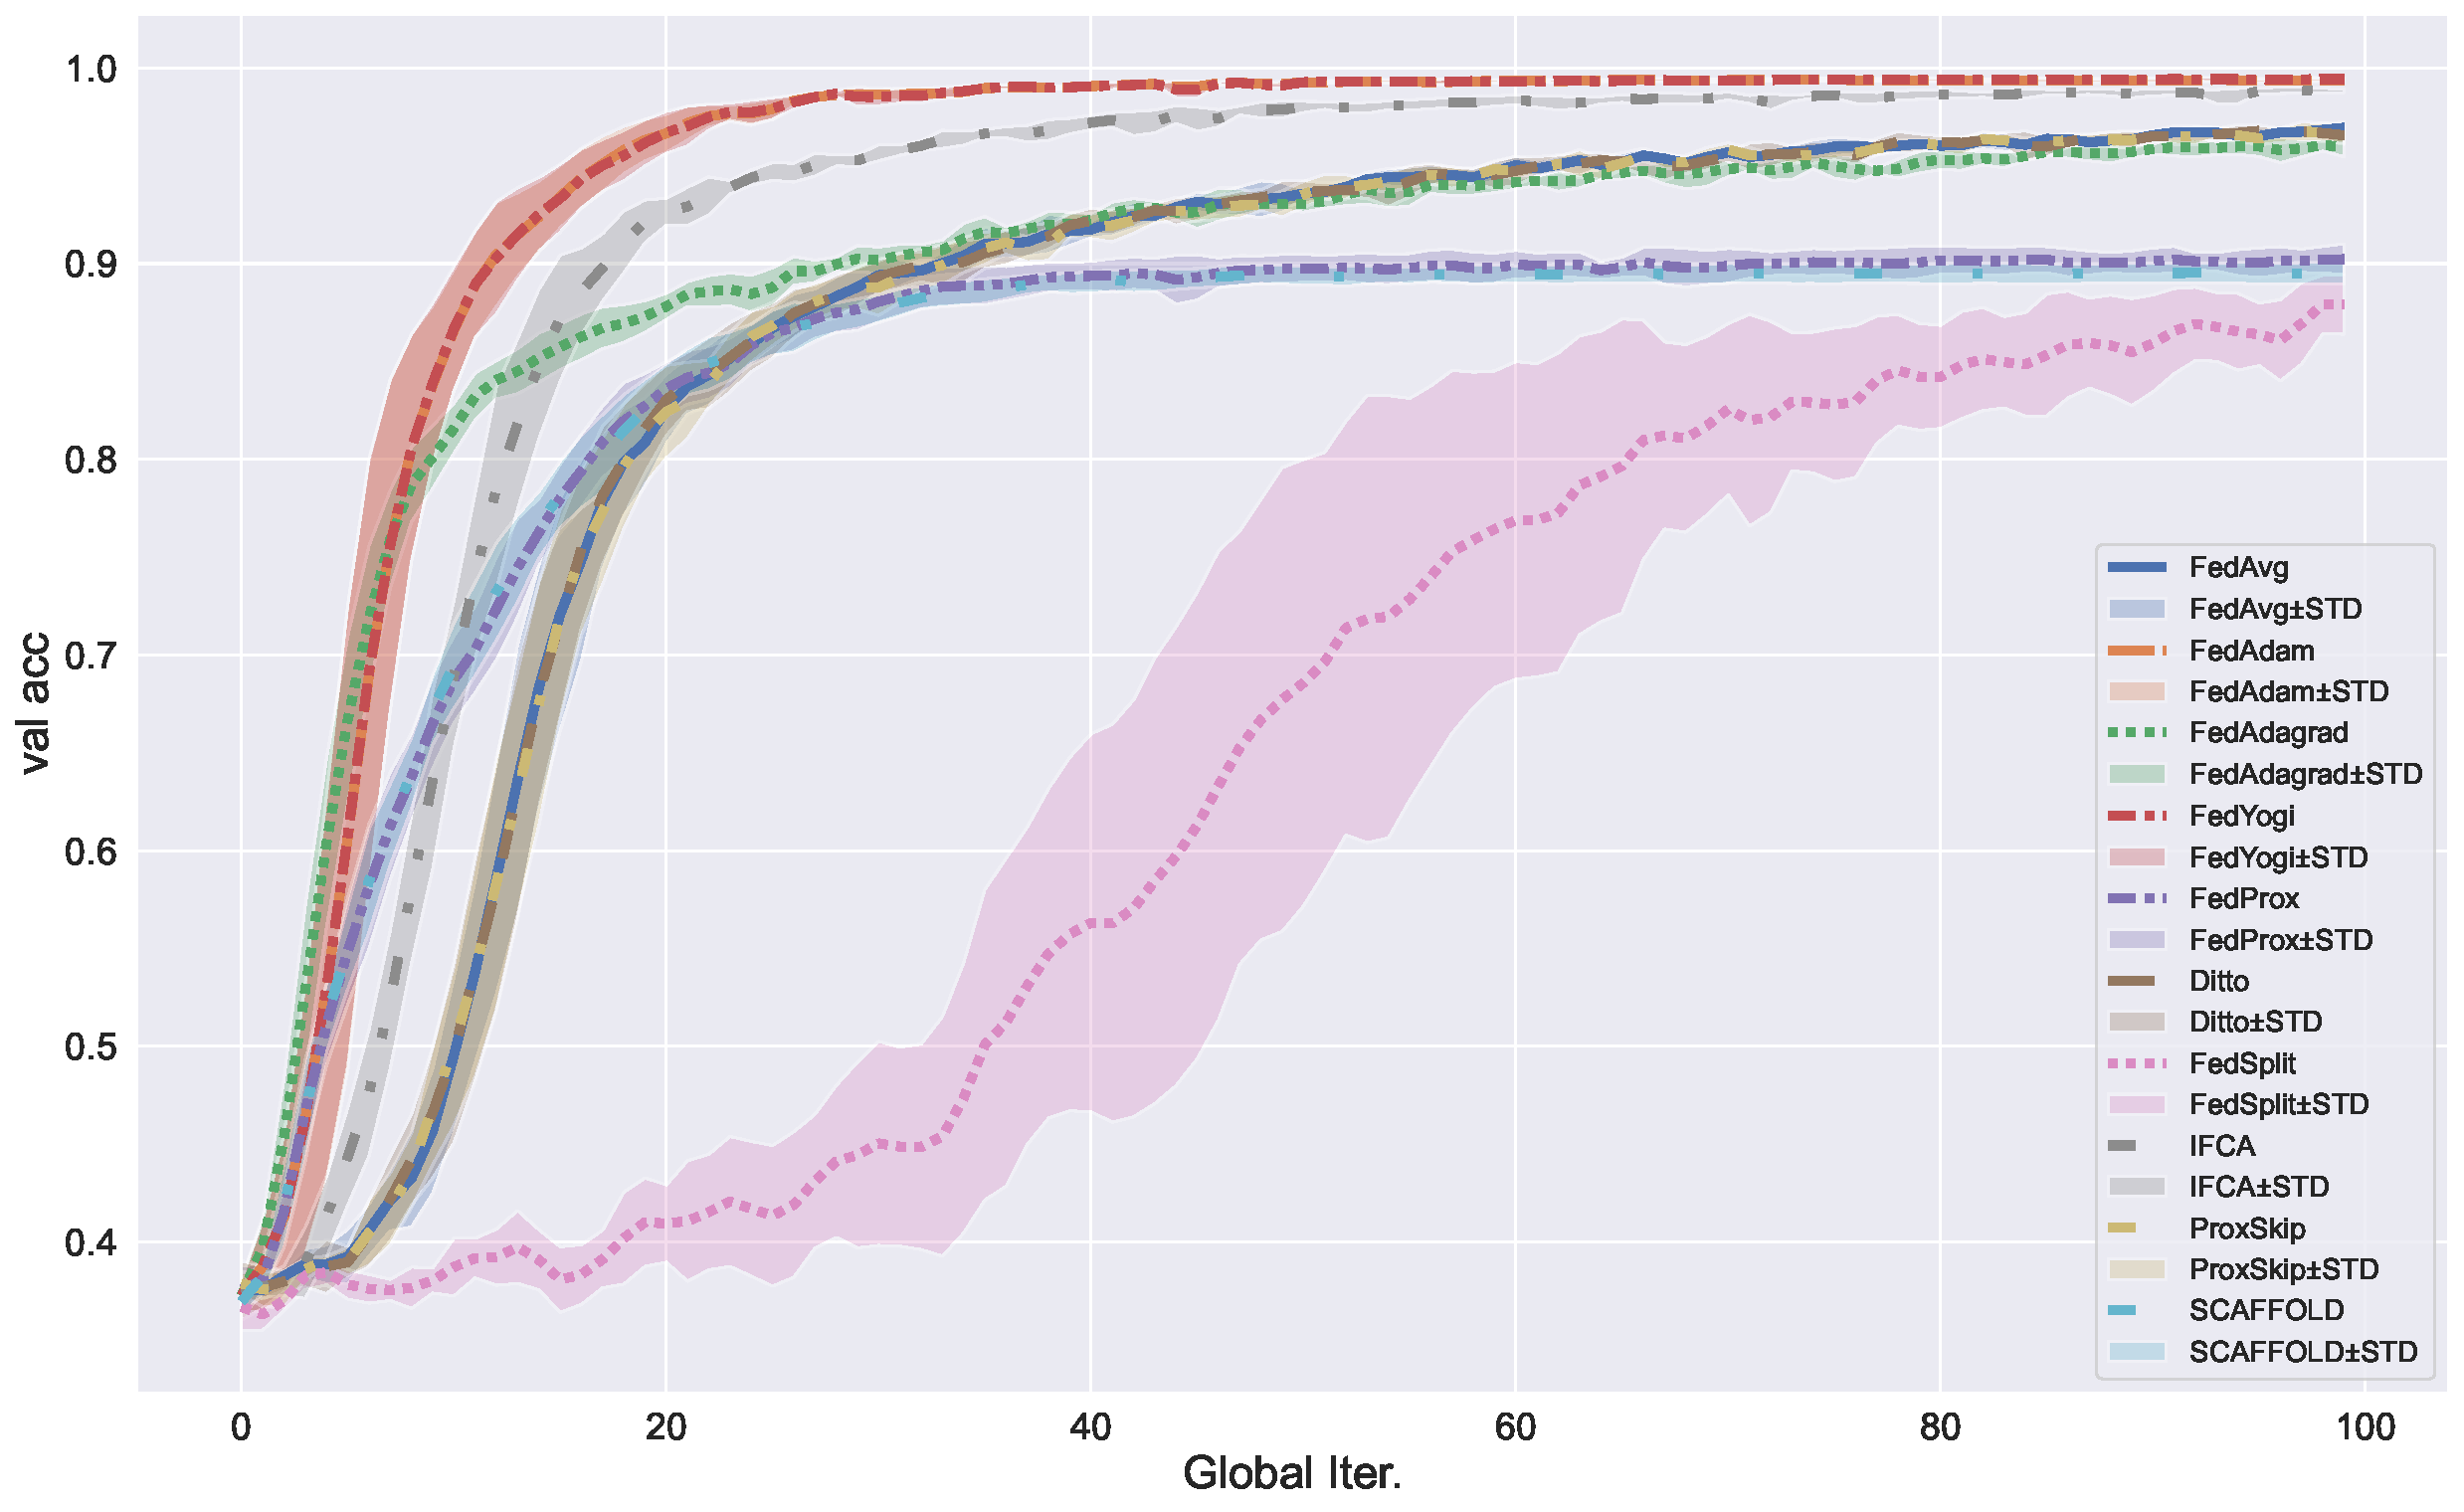
\includegraphics[width=0.9\textwidth]{figures/standard-test-ratio-100-val-acc.pdf}%to upload
    \caption{几种典型的联邦学习算法在子节点训练参与率为$100\%$时,在测试集上的准确率曲线}
    \label{fig:standard-test-ratio-100-val-acc}
\end{figure}

通过这一组数值实验,可以看到,\texttt{FedAdam}, \texttt{FedYogi}算法在设置了合适的全局步长 (关于相关算法全局步长的讨论,详见本章\S\ref{sec:chap6-lr}以及参考文献\parencite{reddi2020fed_opt}附录D.4) 的前提下,在收敛速度、算法效果 (以测试集上准确率计) 、稳定性以及关于子节点参与每轮训练比例的鲁棒性等方面都是十分出色的。有聚类数目先验知识的聚类联邦算法\texttt{IFCA} (注意到在配置文件\ref{lst:fl-sim-config}~中,我们为\texttt{IFCA}算法设置的聚类数目与数据集\texttt{FedProxFEMNIST}天然具有的聚类结构是相匹配的) 在这些方面表现稍次之。在收敛速度、算法效果、稳定性、鲁棒性等方面再次一些的是\texttt{FedAvg}, \texttt{FedAdagrad}, \texttt{Ditto}等算法. 自适应联邦算法\texttt{FedAdam}, \texttt{FedYogi}, \texttt{FedAdagrad}, 以及联邦平均算法\texttt{FedAvg}这几个算法之间的数值比较关系基本与参考文献\parencite{reddi2020fed_opt}第4节以及第5节进行的数值实验结果相符。

\texttt{FedProx}, \texttt{ProxSkip}等算法在收敛速度、算法效果、稳定性、鲁棒性等某些方面与上述算法有一定的差距,特别是关于子节点参与每轮训练比例的鲁棒性等方面。另一个指的关注的问题是,当子节点训练参与率为$100\%$时,跳步算法\texttt{ProxSkip}实际上就是联邦平均算法\texttt{FedAvg},这一点可以从图\ref{fig:standard-test-ratio-100-val-acc}看出。但是当子节点训练参与率低于$100\%$时,跳步算法\texttt{ProxSkip}的鲁棒性明显比联邦平均算法\texttt{FedAvg}低。二者的区别在于,例如当子节点训练参与率等于$30\%$时,跳步算法\texttt{ProxSkip}约定在比例为$30\%$的训练轮次进行子节点与中心节点的通信与全局模型的更新,而在其余训练轮次,所有子节点只进行本地训练,并不与中心节点通信、更新全局模型。联邦平均算法\texttt{FedAvg}则是在每一个训练轮次选取$30\%$的子节点与中心节点通信,利用这部分信息更新全局模型。后者的做法更符合实际的联邦学习场景,并且从数值上看也更加鲁棒。

对于联邦分裂算法\texttt{FedSplit}来说,只有子节点训练参与率达到$100\%$的时候,算法才能收敛。可以从算法伪代码\ref{algo:fedsplit}看到,它并没有考虑每轮迭代只有部分子节点参与的情况,这也是基于算子分裂方法设计的联邦学习算法需要注意的潜在问题。


\section{联邦学习算法关于子节点训练参与率的鲁棒性的数值评测}
\addcontentsline{toe}{section}{{\currentchapter .2\ \ Numerical Evaluation of the Robustness of Federated Learning Algorithms on the Participation Rate of the Clients}\numberline\,}
\label{sec:chap6-sample}

% NOT finished

在上一节中,几种典型的联邦学习算法的数值效果

\begin{figure}[ht]
\centering
\begin{subfigure}{.5\textwidth}
  \centering
  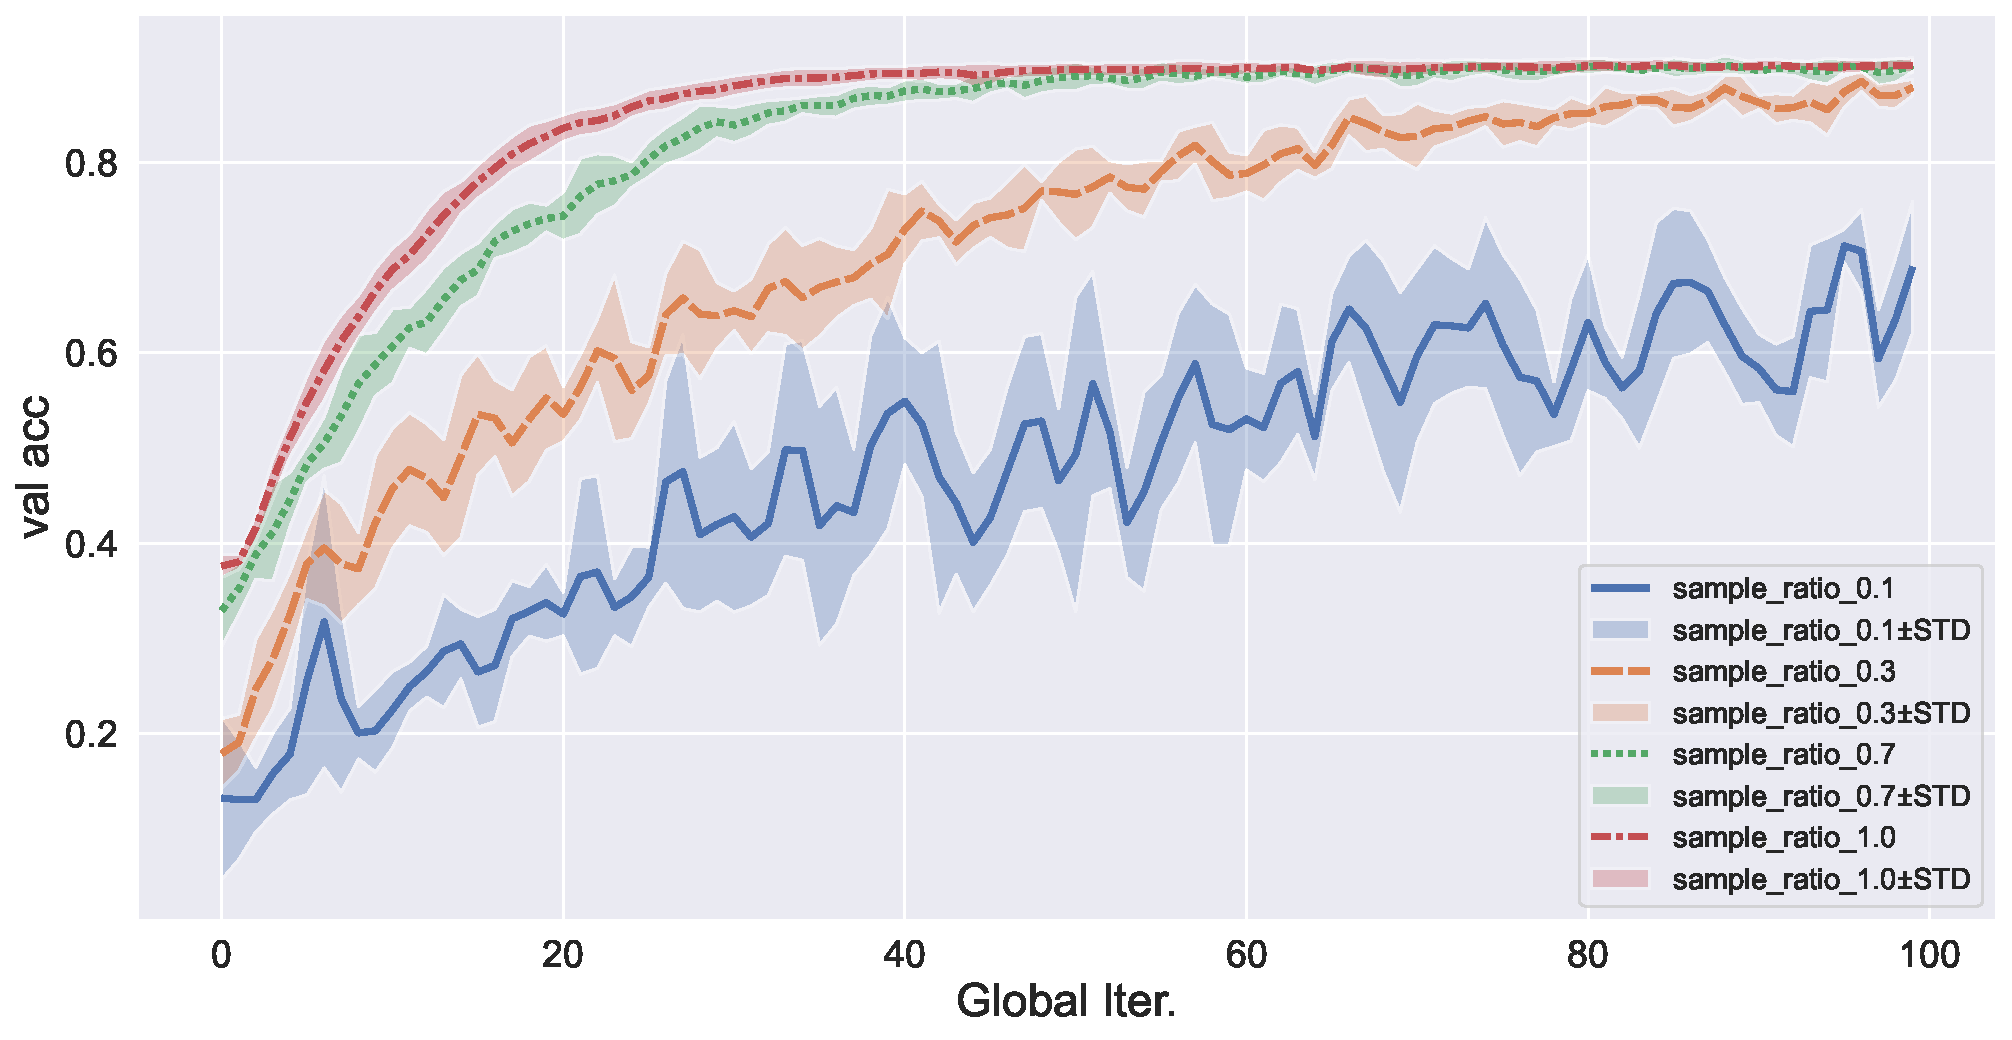
\includegraphics[width=.95\linewidth]{figures/fedprox-compare-sample-ratio-val-acc.pdf}
  \caption{xx}
  \label{fig:fedprox-compare-sample-ratio-val-acc}
\end{subfigure}%
\begin{subfigure}{.5\textwidth}
  \centering
  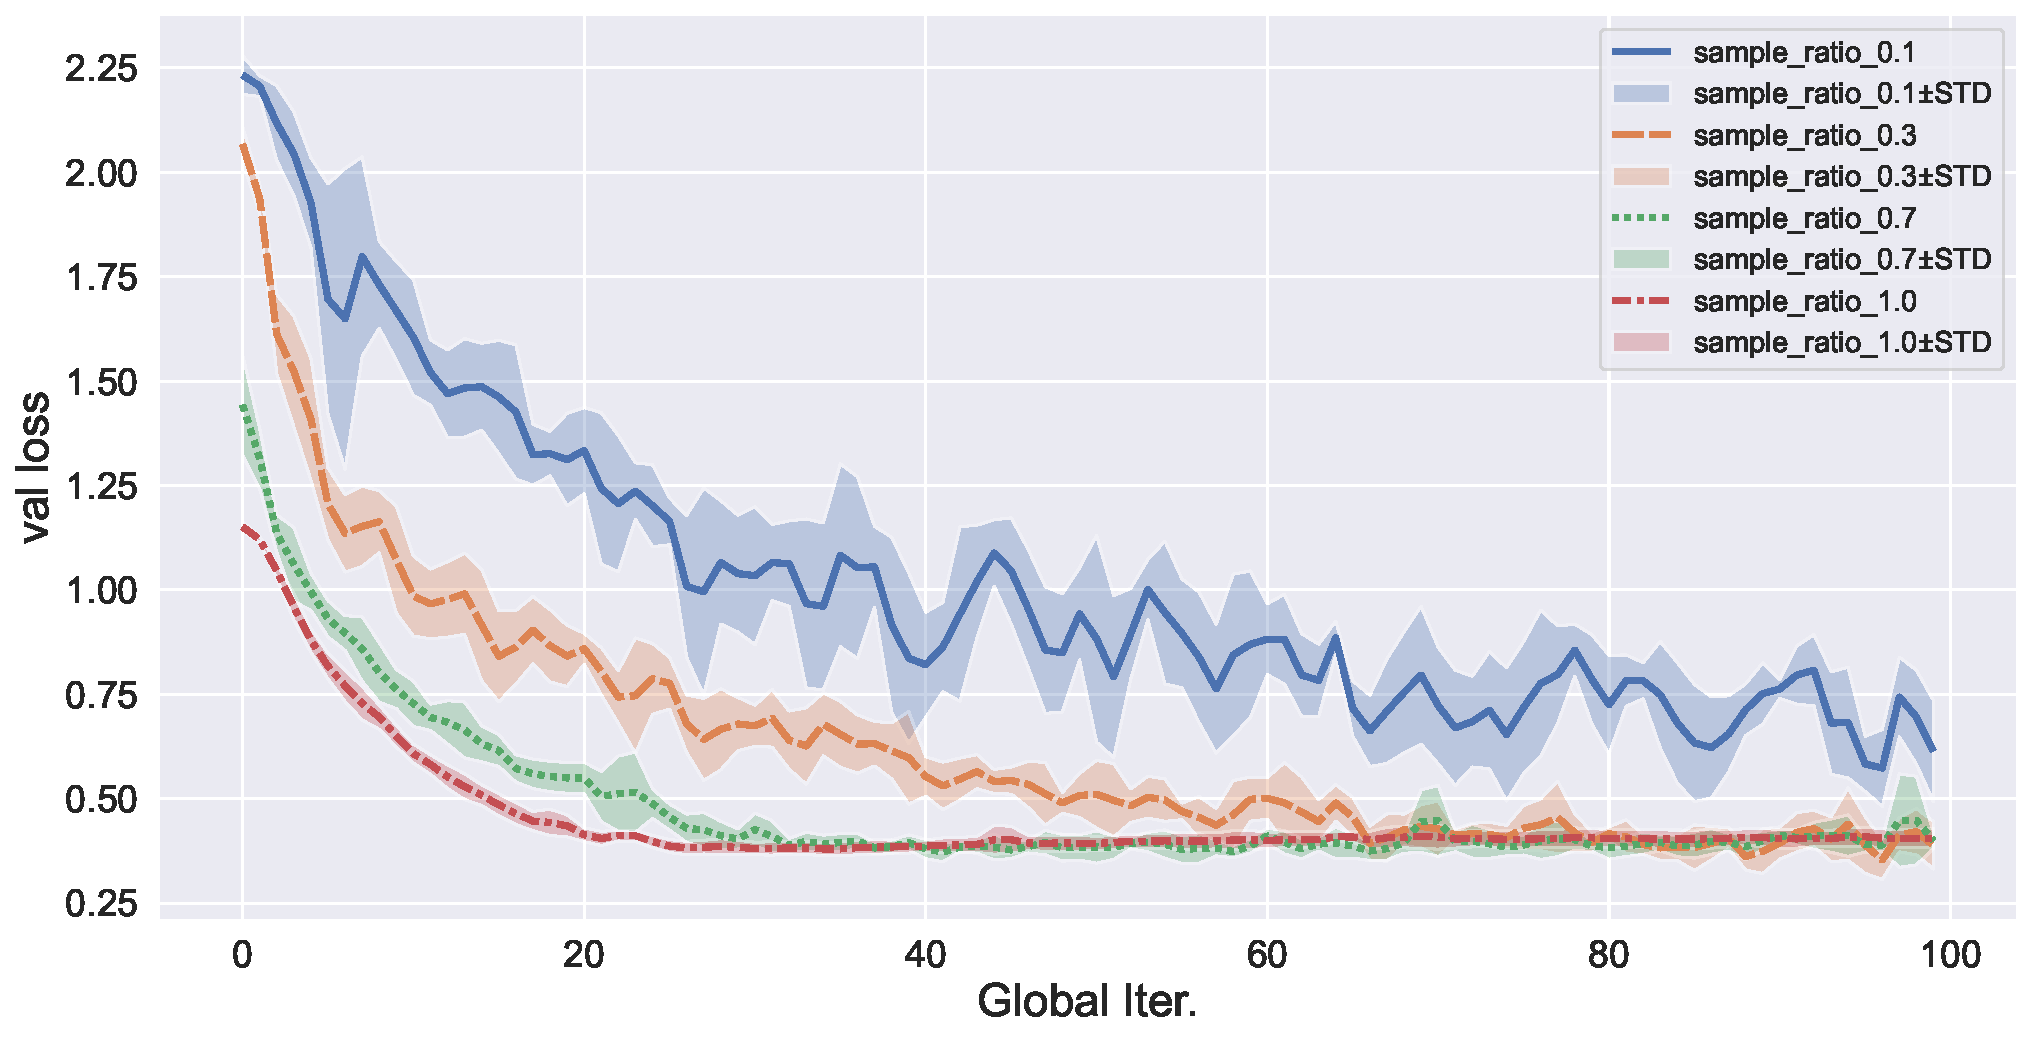
\includegraphics[width=.95\linewidth]{figures/fedprox-compare-sample-ratio-val-loss.pdf}
  \caption{xx}
  \label{fig:fedprox-compare-sample-ratio-val-loss}
\end{subfigure}
\begin{subfigure}{.5\textwidth}
  \centering
  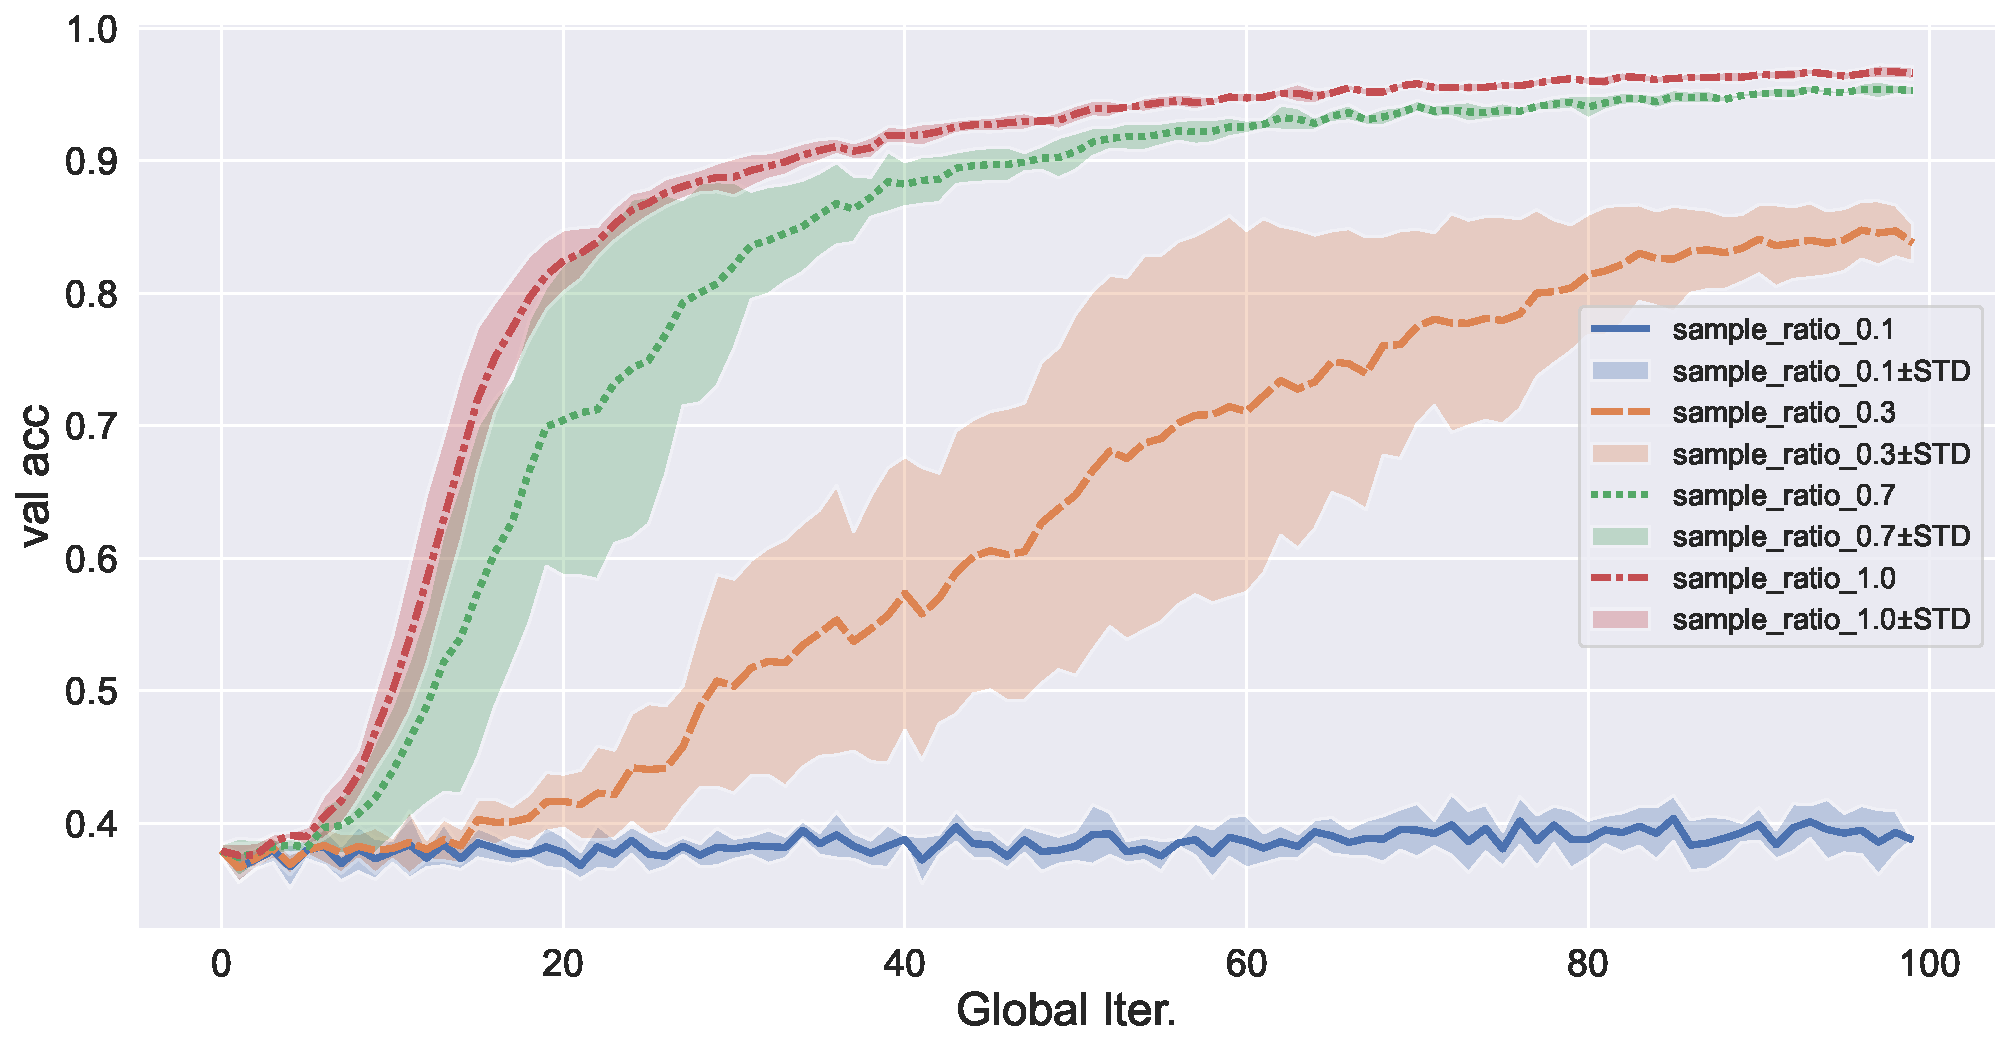
\includegraphics[width=.95\linewidth]{figures/proxskip-compare-sample-ratio-val-acc.pdf}
  \caption{xx}
  \label{fig:proxskip-compare-sample-ratio-val-acc}
\end{subfigure}%
\begin{subfigure}{.5\textwidth}
  \centering
  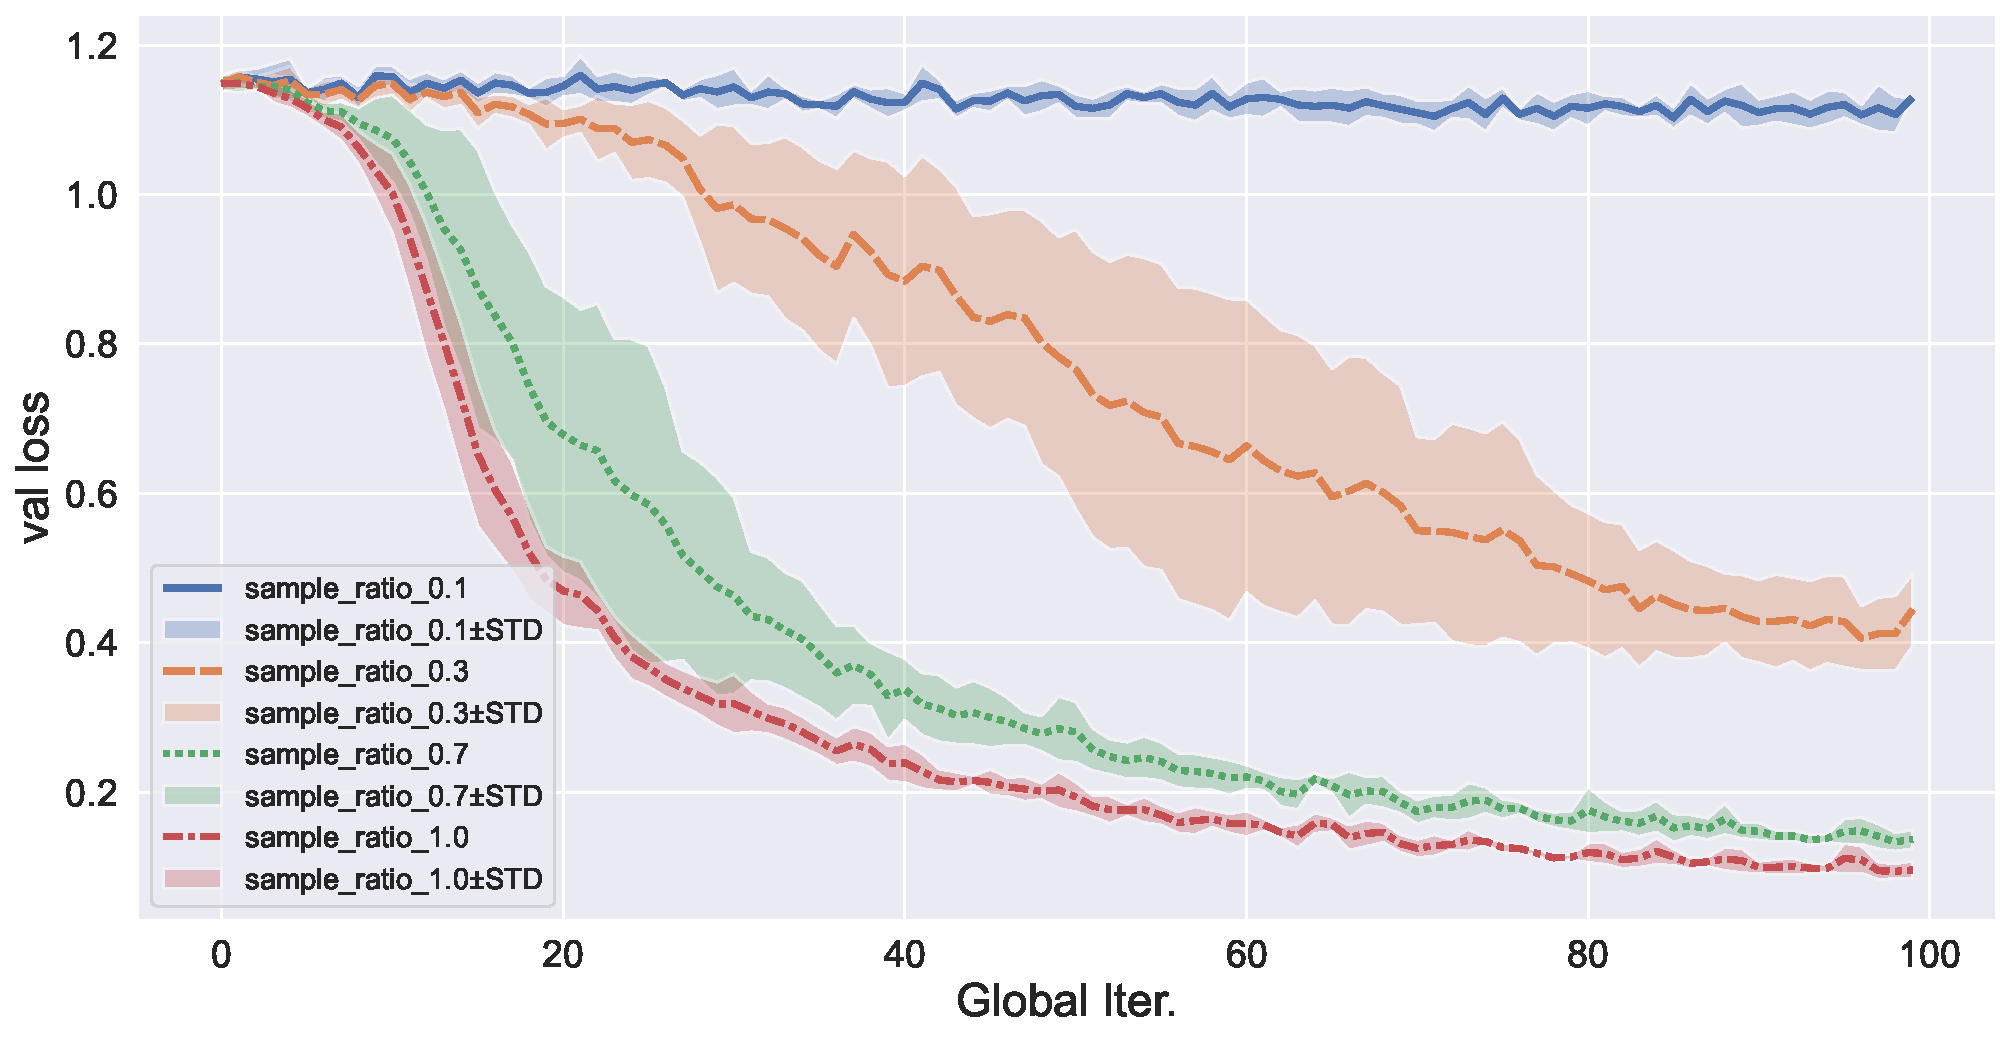
\includegraphics[width=.95\linewidth]{figures/proxskip-compare-sample-ratio-val-loss.pdf}
  \caption{xx}
  \label{fig:proxskip-compare-sample-ratio-val-loss}
\end{subfigure}
\begin{subfigure}{.5\textwidth}
  \centering
  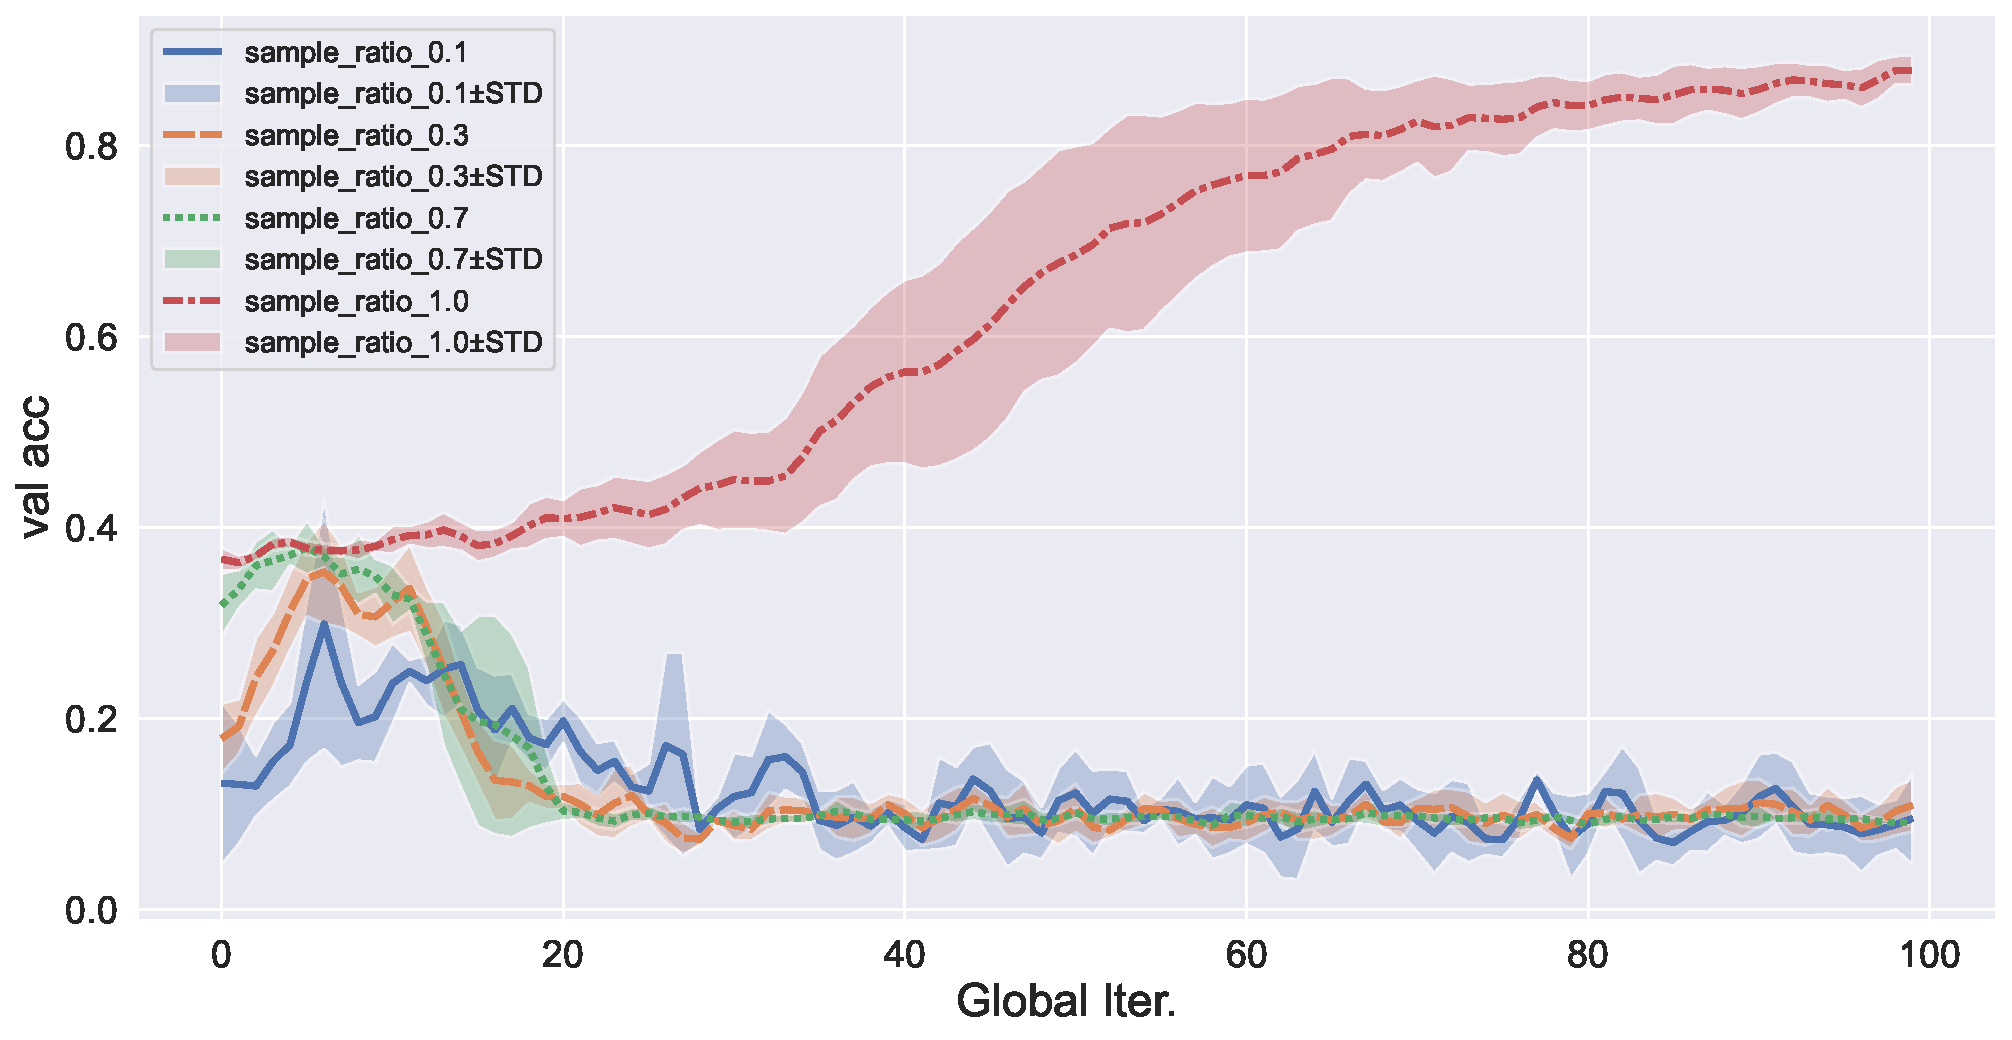
\includegraphics[width=.95\linewidth]{figures/fedsplit-compare-sample-ratio-val-acc.pdf}
  \caption{xx}
  \label{fig:fedsplit-compare-sample-ratio-val-acc}
\end{subfigure}%
\begin{subfigure}{.5\textwidth}
  \centering
  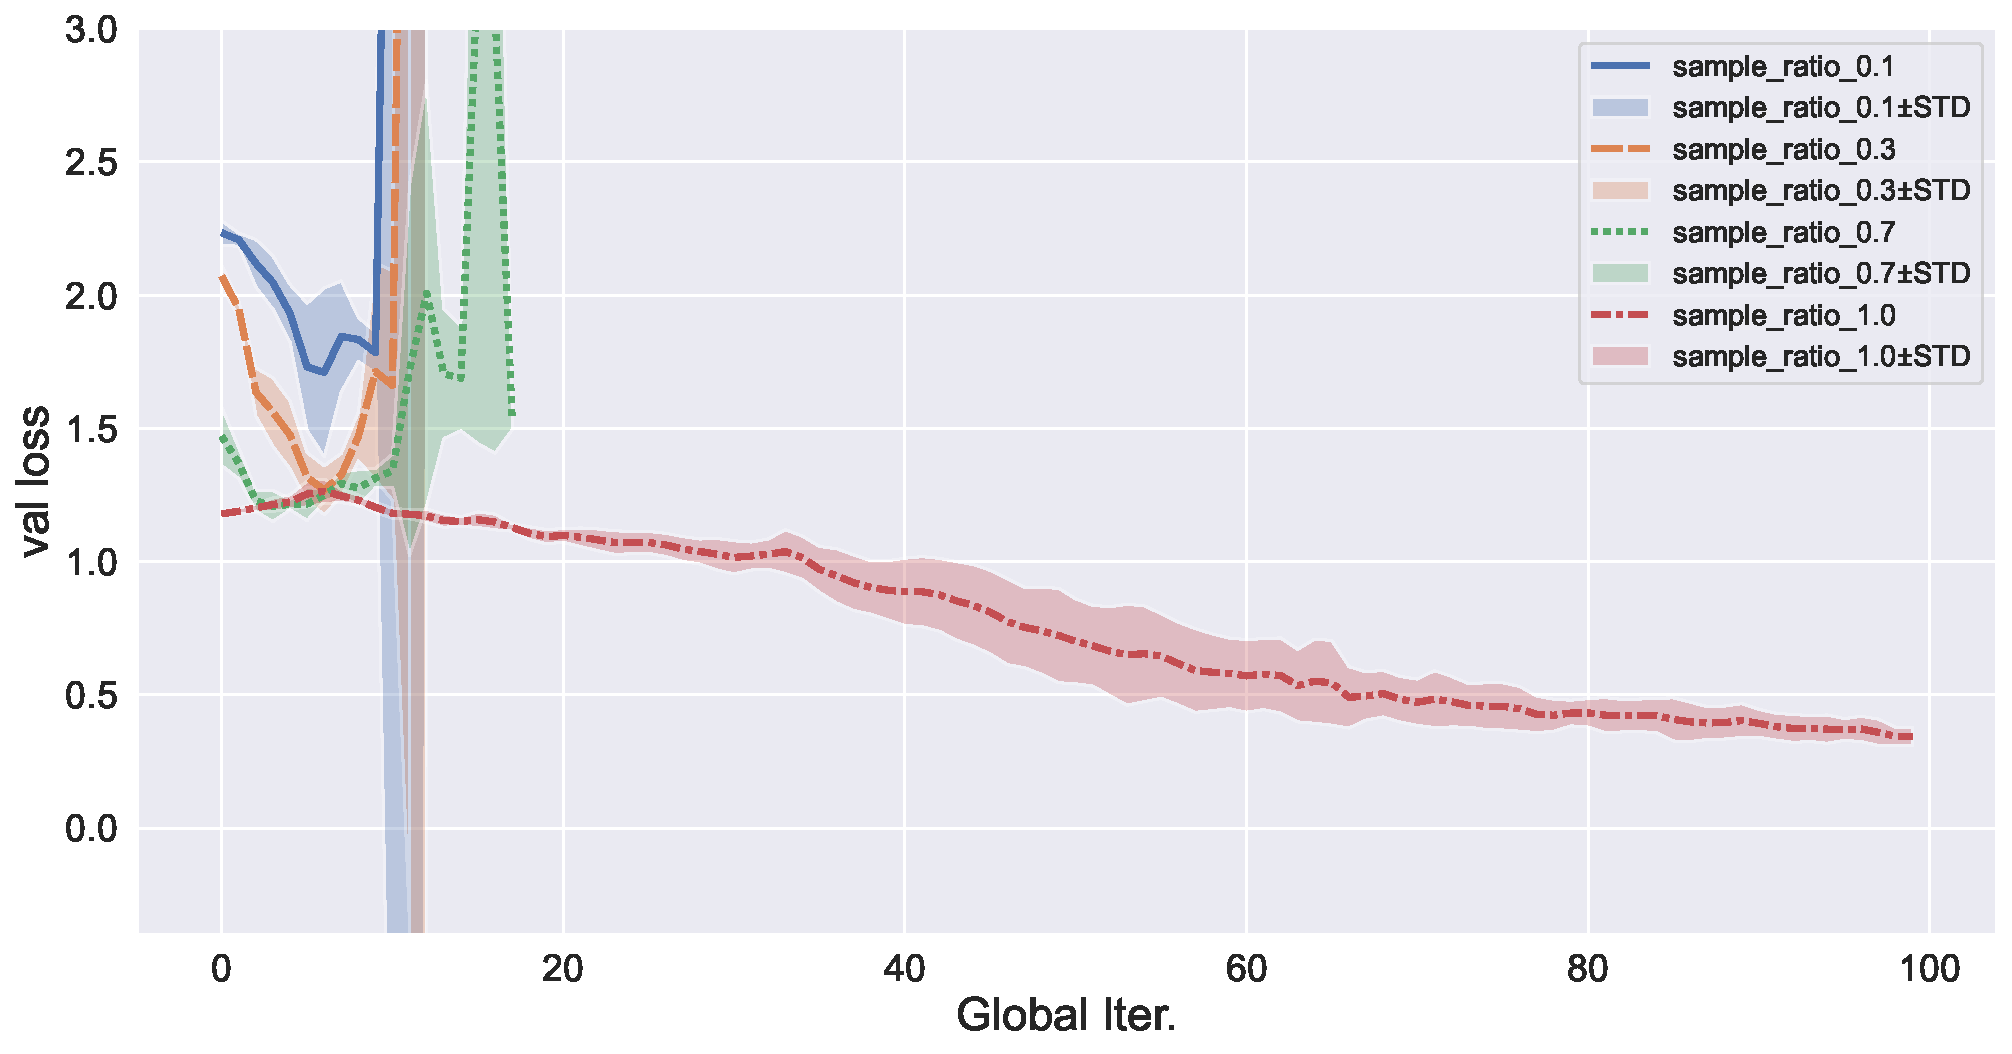
\includegraphics[width=.95\linewidth]{figures/fedsplit-compare-sample-ratio-val-loss.pdf}
  \caption{xx}
  \label{fig:fedsplit-compare-sample-ratio-val-loss}
\end{subfigure}
\begin{subfigure}{.5\textwidth}
  \centering
  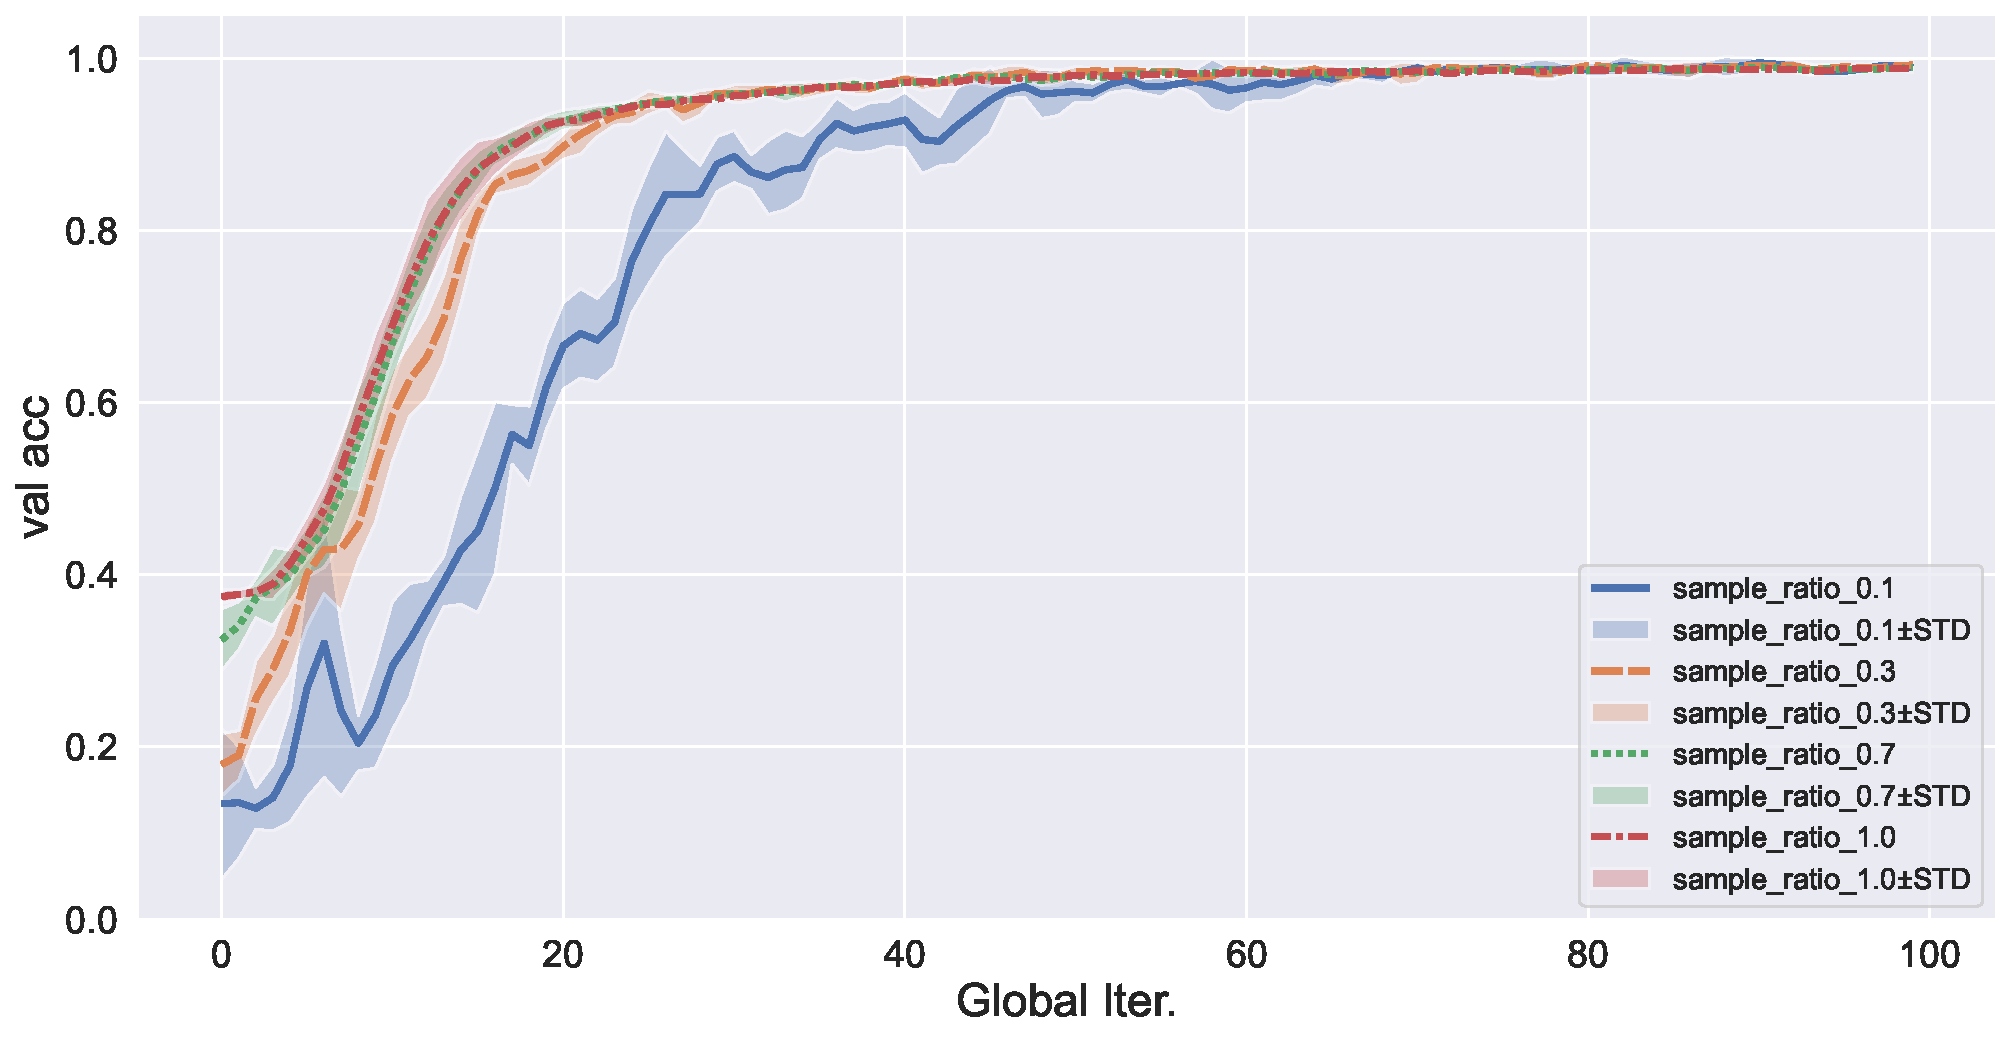
\includegraphics[width=.95\linewidth]{figures/ifca-compare-sample-ratio-val-acc.pdf}
  \caption{xx}
  \label{fig:ifca-compare-sample-ratio-val-acc}
\end{subfigure}%
\begin{subfigure}{.5\textwidth}
  \centering
  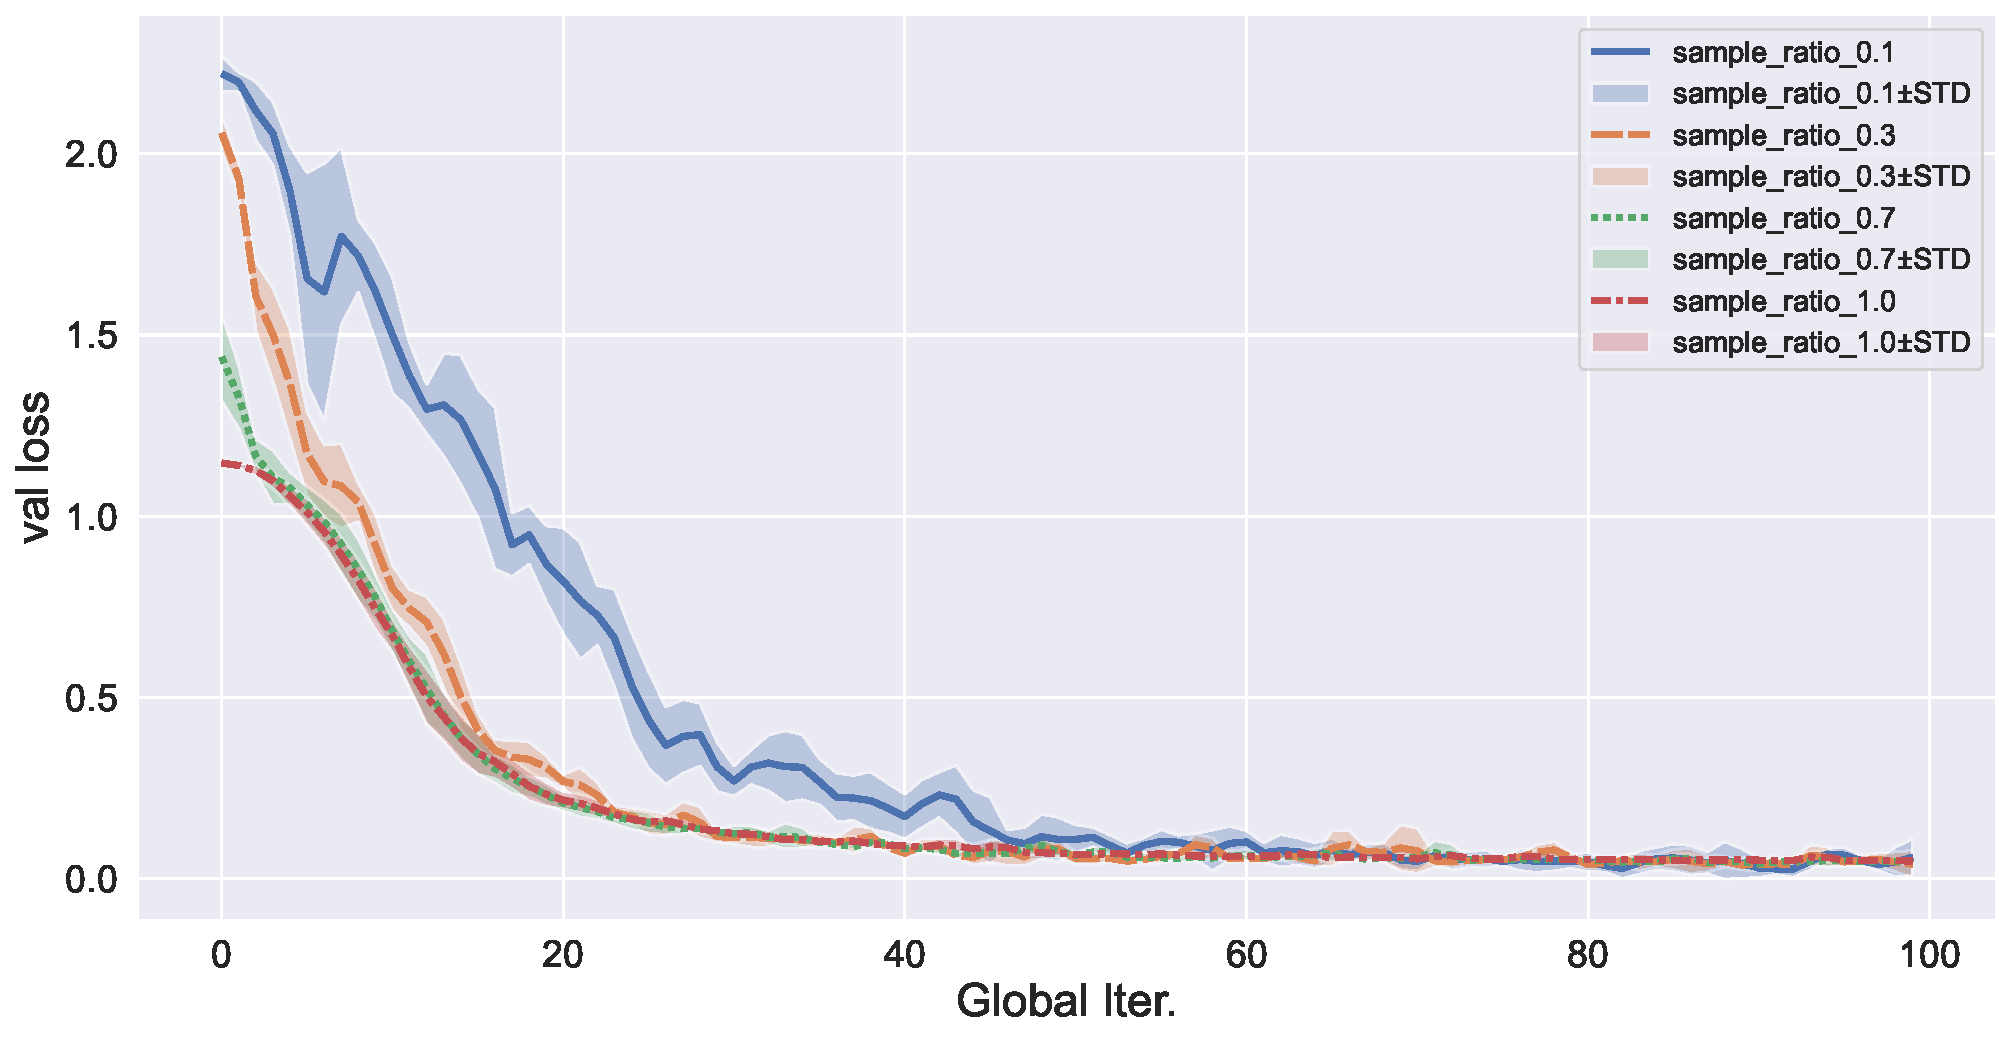
\includegraphics[width=.95\linewidth]{figures/ifca-compare-sample-ratio-val-loss.pdf}
  \caption{xx}
  \label{fig:ifca-compare-sample-ratio-val-loss}
\end{subfigure}
\caption{xx}
\label{fig:fedprox-compare-sample-ratio}
\end{figure}



待写。。。。


\section{几类自适应联邦学习算法关于学习率敏感性的数值结果}
\addcontentsline{toe}{section}{{\thecurrentchapter .3\ \ Numerical Results on Learning Rate Sensitivity of Several Adaptive Federated Learning Algorithms}\numberline\,}
\label{sec:chap6-lr}

% almost finished

我们已经在本章的\S\ref{sec:chap6-overall}观察到了,联邦自适应类算法\texttt{FedAdam}, \texttt{FedYogi}, \texttt{FedAdagrad}有不错的数值效果,同时对于高比例的子节点掉队者这样的极端场景也有着极强的鲁棒性。但是这些联邦学习算法也有比较敏感的超参数,即中心节点上的全局学习率。图图\ref{fig:standard-test-ratio-10-val-acc}, \ref{fig:standard-test-ratio-30-val-acc}, \ref{fig:standard-test-ratio-70-val-acc}, \ref{fig:standard-test-ratio-100-val-acc}~对应的数值实验将联邦自适应类算法\texttt{FedAdam}, \texttt{FedYogi}, \texttt{FedAdagrad}的全局学习率设置为了$0.003 \approx 10^{-2.5}$ (见配置文件\ref{lst:fl-sim-config}). 为了探究这几个联邦自适应类算法对于全局学习率的敏感性,我们额外进行了几组试验,固定子节点的训练参与率为$30\%,$ 并分别将全局学习率设置为$10^{-2}$以及$10^{-3}.$ 相关的结果整理、绘制在了图\ref{fig:fedopt-sample-30-compare-lr-val-acc}~中。

\begin{figure}[ht]
\centering
\begin{subfigure}{.5\textwidth}
  \centering
  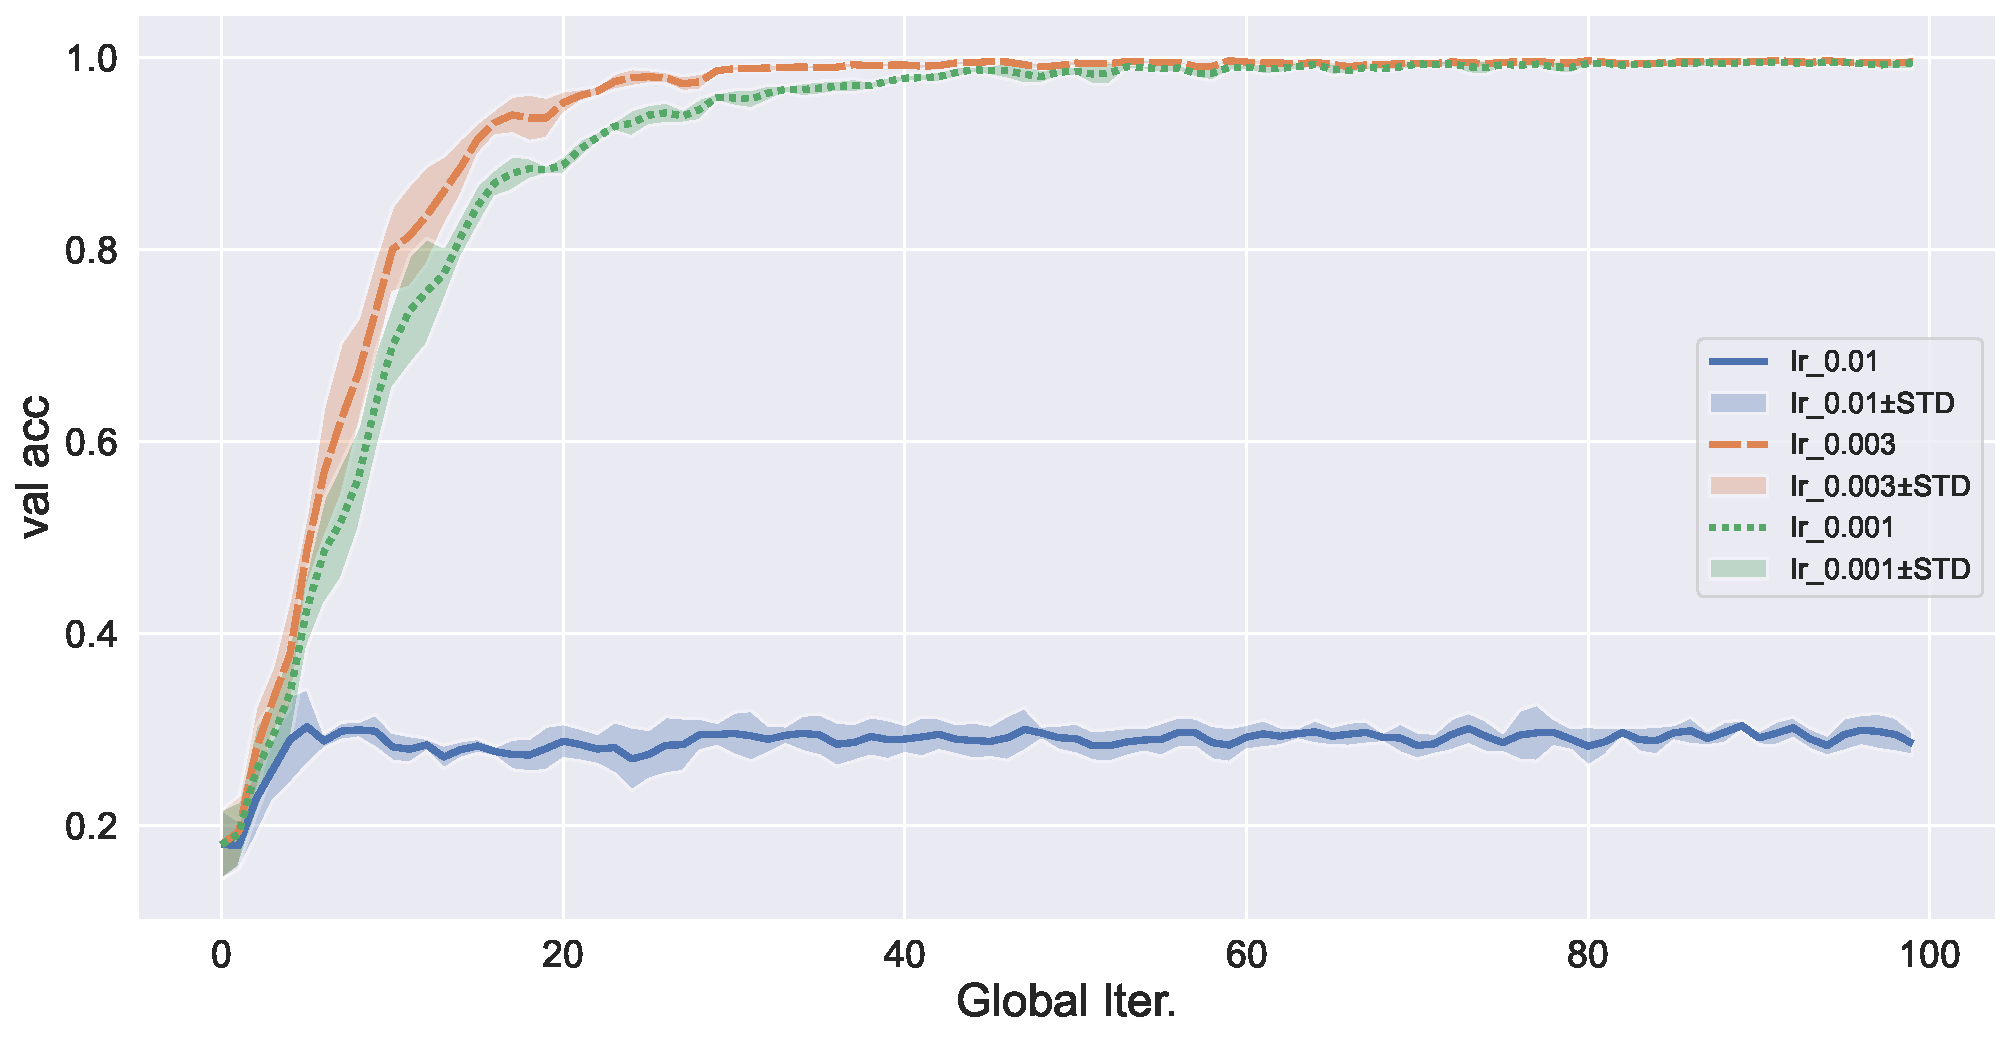
\includegraphics[width=.95\linewidth]{figures/adam-sample-30-compare-lr-val-acc.pdf}
  \caption{\texttt{FedAdam}算法在不同全局学习率下测试集上的准确率曲线}
  \label{fig:adam-sample-30-compare-lr-val-acc}
\end{subfigure}%
\begin{subfigure}{.5\textwidth}
  \centering
  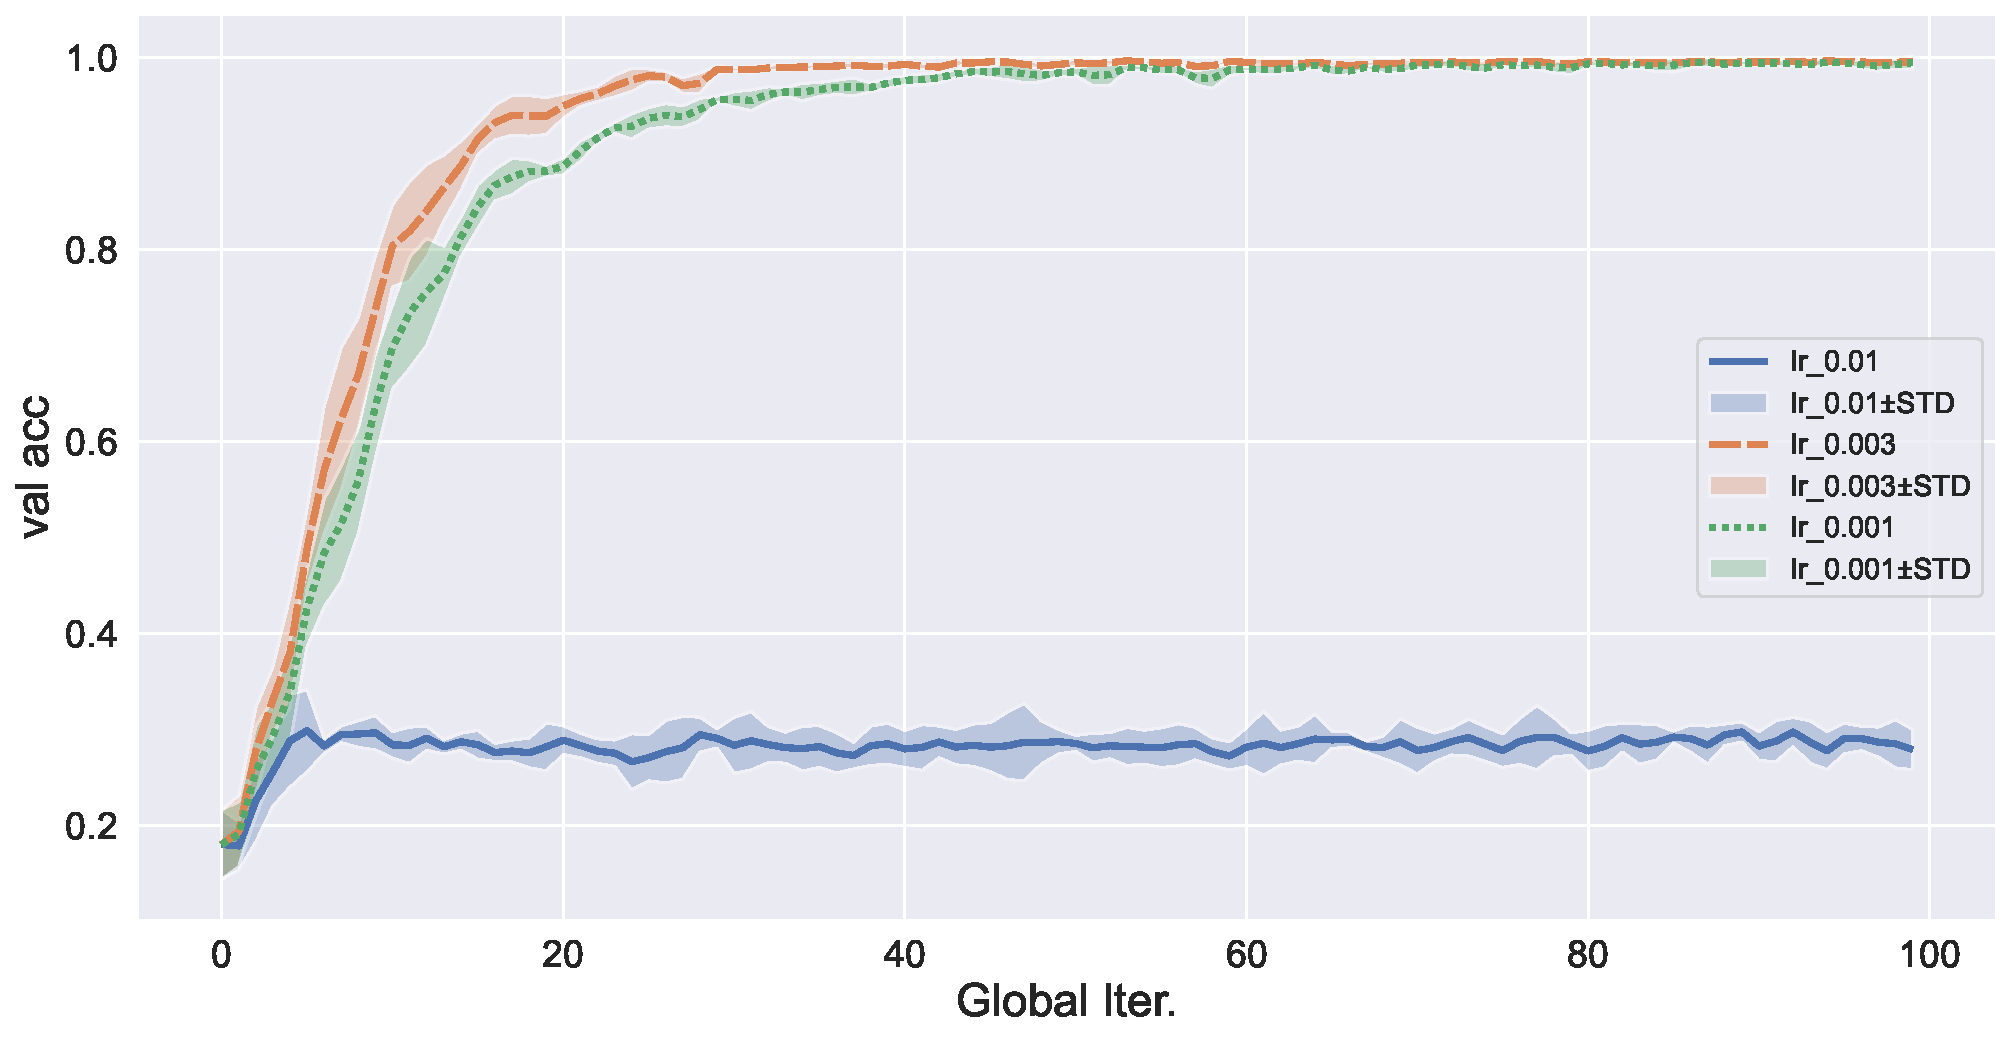
\includegraphics[width=.95\linewidth]{figures/yogi-sample-30-compare-lr-val-acc.pdf}
  \caption{\texttt{FedYogi}算法在不同全局学习率下测试集上的准确率曲线}
  \label{fig:yogi-sample-30-compare-lr-val-acc}
\end{subfigure}
\begin{subfigure}{.6\textwidth}
  \centering
  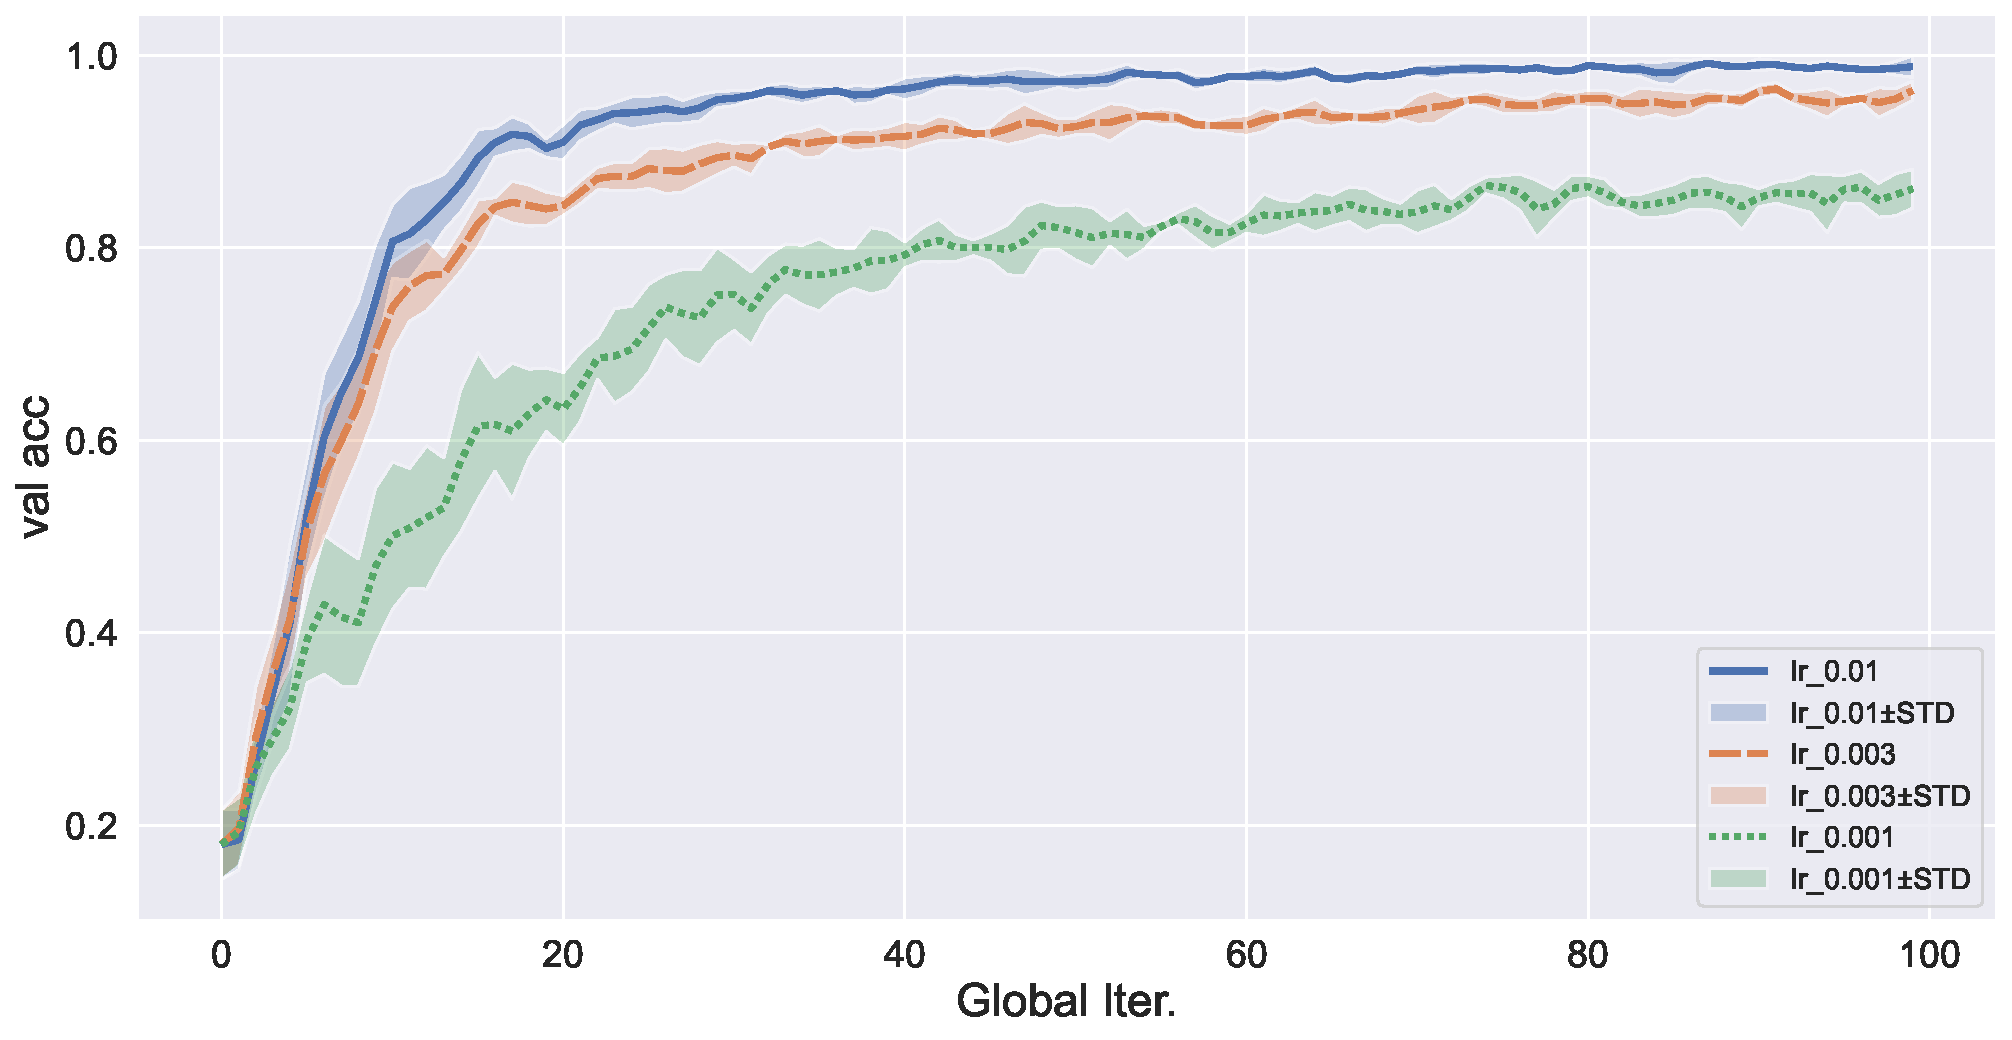
\includegraphics[width=.95\linewidth]{figures/adagrad-sample-30-compare-lr-val-acc.pdf}
  \caption{\texttt{FedAdagrad}算法在不同全局学习率下测试集上的准确率曲线}
  \label{fig:adagrad-sample-30-compare-lr-val-acc}
\end{subfigure}
\caption{几种联邦自适应类算法在不同全局学习率下测试集上的准确率曲线,子节点的训练参与率固定为$30\%$}
\label{fig:fedopt-sample-30-compare-lr-val-acc}
\end{figure}

可以看到,对于联邦自适应算法\texttt{FedAdam}与\texttt{FedYogi}来说,在$10^{-2}, 10^{-2.5}, 10^{-3}$这几个全局学习率中,最适合的是$10^{-2.5},$ 但是稍小的学习率$10^{-3}$只是稍微降低了算法的收敛速度,但并没降低算法的数值效果 (在测试集上的准确率)。联邦自适应算法\texttt{FedAdagrad}对于全局学习率这一超参数没有\texttt{FedAdam}与\texttt{FedYogi}这么敏感,但是其代价是,更小的学习率降低了算法的数值效果。

为了排除子节点的训练参与率对于这几种联邦自适应类算法对全局学习率敏感性的影响,对于子节点的训练参与率$10\%, 70\%, 100\%$我们都做了类似的数值实验,并且得到了相似的数值结果。唯一的例外是,当子节点的训练参与率被设置为$70\%,$ 并且随机数种子置为$0$时,\texttt{FedAdam}算法在全局学习率置为$10^{-2}$时得到了相同的 (相同指的是,试验在测试集上的最终准确率) 收敛的结果。相关的数值结果绘制在图\ref{fig:adam-sample-70-compare-lr-val-acc}~中。

\begin{figure}[ht]
    \centering
    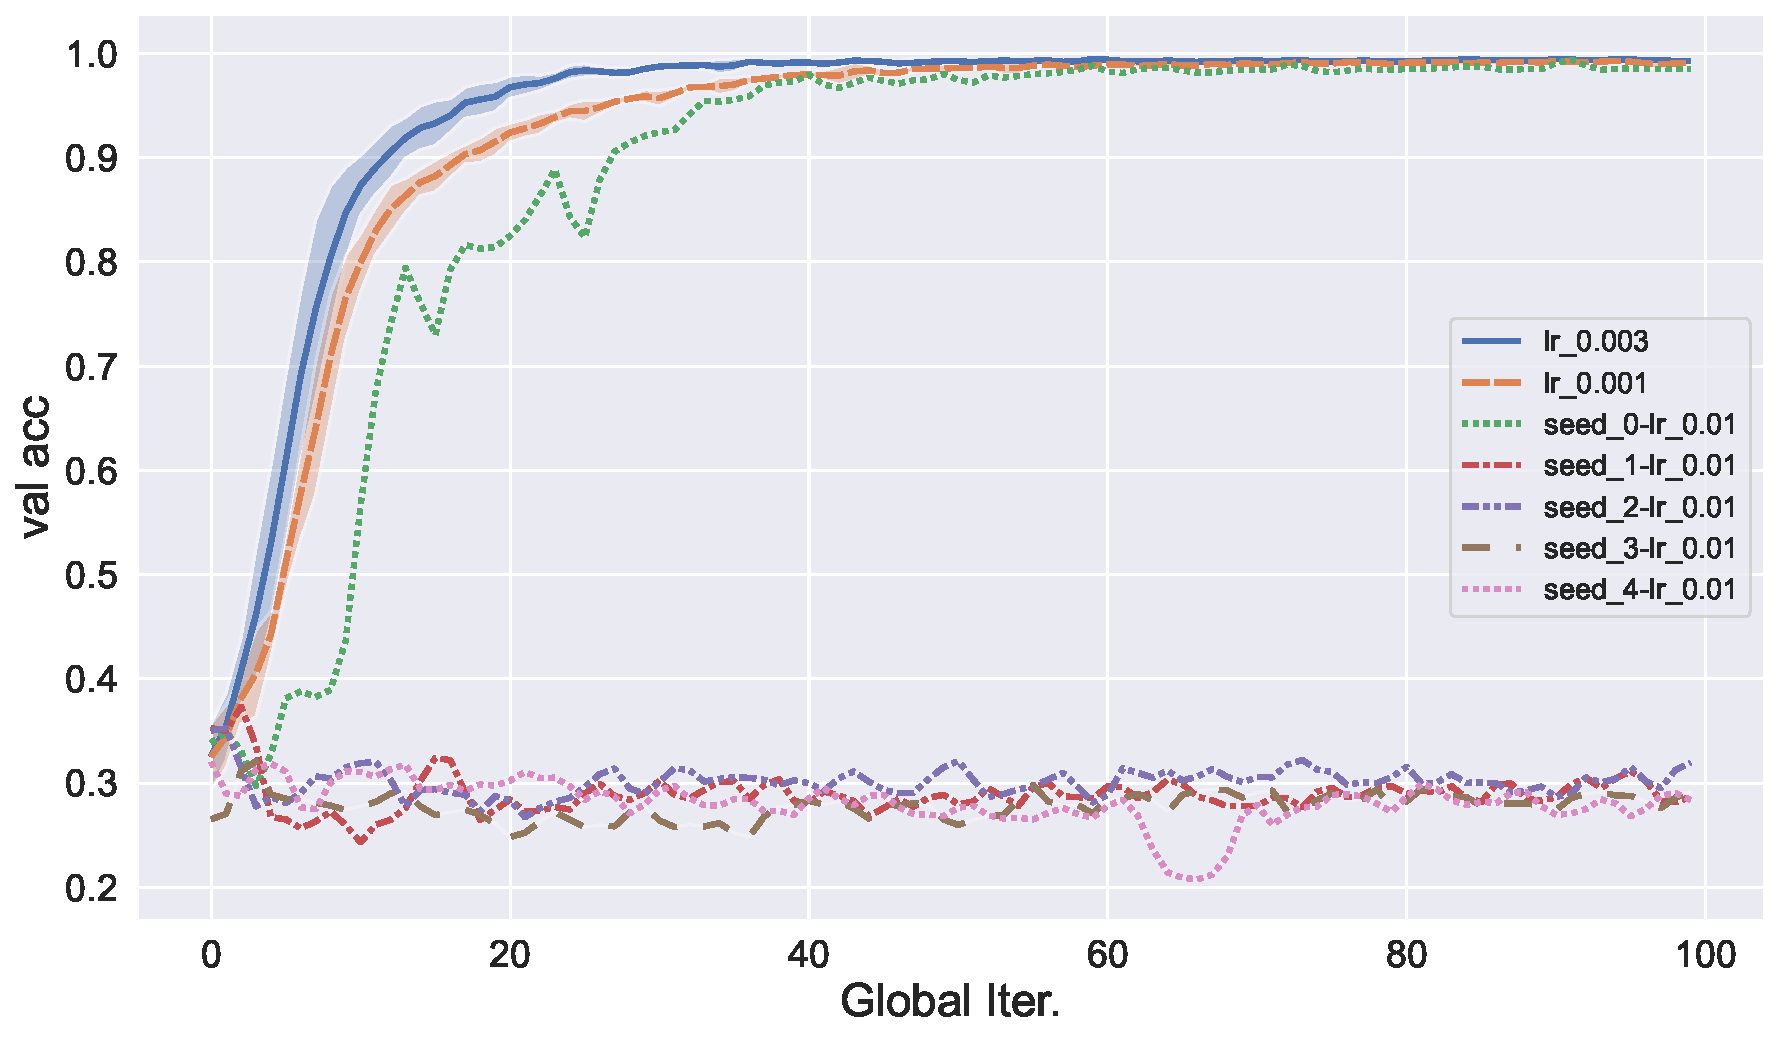
\includegraphics[width=0.6\textwidth]{figures/adam-sample-70-compare-lr-val-acc.pdf}
    \caption{\texttt{FedAdam}算法在不同全局学习率下测试集上的准确率曲线,子节点的训练参与率固定为$70\%$}
    \label{fig:adam-sample-70-compare-lr-val-acc}
\end{figure}

